% TODO Change language to en_GB (recommended) or en_US for English documents
\documentclass[11pt,a4paper,oneside]{report}             % Single-side
%\documentclass[11pt,a4paper,twoside,openright]{report}  % Duplex

% thanks to http://tex.stackexchange.com/a/47579/71109
\usepackage{ifxetex}
\usepackage{ifluatex}
\newif\ifxetexorluatex % a new conditional starts as false
\ifnum 0\ifxetex 1\fi\ifluatex 1\fi>0
   \xetexorluatextrue
\fi

\ifxetexorluatex
  \usepackage{fontspec}
\else
  \usepackage[T1]{fontenc}
  \usepackage[utf8]{inputenc}
  \usepackage[lighttt]{lmodern}
  \ttfamily\DeclareFontShape{T1}{lmtt}{m}{it}{<->sub*lmtt/m/sl}{}
\fi

\usepackage[english,magyar]{babel} % Alapértelmezés szerint utoljára definiált nyelv lesz aktív, de később külön beállítjuk az aktív nyelvet.

\usepackage{emptypage} % omit page number on empty pages

%\usepackage{cmap}
\usepackage{amsfonts,amsmath,amssymb} % Mathematical symbols.
\usepackage[ruled,boxed,resetcount,linesnumbered]{algorithm2e} % For pseudocodes. % beware: this is not compatible with LuaLaTeX, see http://tex.stackexchange.com/questions/34814/lualatex-and-algorithm2e
\usepackage{booktabs} % For publication quality tables for LaTeX
\usepackage{graphicx}

%\usepackage{fancyhdr}
%\usepackage{lastpage}

\usepackage{geometry}
%\usepackage{sectsty}
\usepackage{setspace} % For setting line spacing

\usepackage[unicode]{hyperref} % For hyperlinks in the generated document.
\usepackage{xcolor}
\usepackage{listings} % For source code snippets.

\usepackage[amsmath,thmmarks]{ntheorem} % Theorem-like environments.

\usepackage[hang]{caption}

\singlespacing

\newcommand{\selecthungarian}{
	\selectlanguage{magyar}
	\setlength{\parindent}{2em}
	\setlength{\parskip}{0em}
	\frenchspacing
}

\newcommand{\selectenglish}{
	\selectlanguage{english}
	\setlength{\parindent}{0em}
	\setlength{\parskip}{0.5em}
	\nonfrenchspacing
	\renewcommand{\figureautorefname}{Figure}
	\renewcommand{\tableautorefname}{Table}
	\renewcommand{\partautorefname}{Part}
	\renewcommand{\chapterautorefname}{Chapter}
	\renewcommand{\sectionautorefname}{Section}
	\renewcommand{\subsectionautorefname}{Section}
	\renewcommand{\subsubsectionautorefname}{Section}
}

\usepackage[numbers]{natbib}
\usepackage{xspace}

\usepackage[colorinlistoftodos,prependcaption,textsize=tiny]{todonotes}

\usepackage{tikz-qtree-compat}
\usepackage{tikz}
\usetikzlibrary{shapes.misc}
\usetikzlibrary{decorations.markings}
\usetikzlibrary{positioning}
\tikzset{cross/.style={cross out, draw, 
         minimum size=2*(#1-\pgflinewidth), 
         inner sep=0pt, outer sep=0pt}}

\usepackage{subcaption}

%TODO Set the main variables
\newcommand{\vikszerzoVezeteknev}{S\'{a}ri}
\newcommand{\vikszerzoKeresztnev}{L\'{a}szl\'{o}}


\newcommand{\vikkonzulensAMegszolitas}{dr.~}
\newcommand{\vikkonzulensAVezeteknev}{Szegletes}
\newcommand{\vikkonzulensAKeresztnev}{Luca}

\newcommand{\vikkonzulensBMegszolitas}{}
\newcommand{\vikkonzulensBVezeteknev}{}
\newcommand{\vikkonzulensBKeresztnev}{}

\newcommand{\vikkonzulensCMegszolitas}{}
\newcommand{\vikkonzulensCVezeteknev}{}
\newcommand{\vikkonzulensCKeresztnev}{}

\newcommand{\vikcim}{Subgraph ismorphism in dynamic graphs} % Cím
\newcommand{\viktanszek}{\bmemit} % Tanszék
\newcommand{\vikdoktipus}{\bsc} % Dokumentum típusa (\bsc vagy \msc)
\newcommand{\vikmunkatipusat}{szakdolgozatot} % a "hallgató nyilatkozat" részhez: szakdolgozatot vagy diplomatervet

%--------------------------------------------------------------------------------------
% TDK-specifikus változók
%--------------------------------------------------------------------------------------
\newcommand{\tdkszerzoB}{Második Szerző} % Második szerző neve; hagyd üresen, ha egyedül írtad a TDK-t.
\newcommand{\tdkev}{2014} % A dolgozat írásának éve (pl. "2014") (Ez OTDK-nál eltérhet az aktuális évtől.)

% További adatok az OTDK címlaphoz (BME-s TDK-hoz nem kell kitölteni)
\newcommand{\tdkevfolyamA}{IV} % Első szerző évfolyama, római számmal (pl. IV).
\newcommand{\tdkevfolyamB}{III} % Második szerző évfolyama, római számmal (pl. III).
\newcommand{\tdkkonzulensbeosztasA}{egyetemi tanár} % Első konzulens beosztása (pl. egyetemi docens)
\newcommand{\tdkkonzulensbeosztasB}{doktorandusz} % Második konzulens beosztása (pl. egyetemi docens)

% \newcommand{\szerzoMeta}{\vikszerzoVezeteknev{} \vikszerzoKeresztnev} % egy szerző esetén
\newcommand{\szerzoMeta}{\vikszerzoVezeteknev{} \vikszerzoKeresztnev, \tdkszerzoB} % két szerző esetén


%TODO Language configuration -- choose one
% Beállítások magyar nyelvű dolgozathoz
% %--------------------------------------------------------------------------------------
% Elnevezések
%--------------------------------------------------------------------------------------
\newcommand{\bme}{Budapesti Műszaki és Gazdaságtudományi Egyetem}
\newcommand{\vik}{Villamosmérnöki és Informatikai Kar}

\newcommand{\bmemit}{Méréstechnika és Információs Rendszerek Tanszék}

\newcommand{\keszitette}{Készítette}
\newcommand{\konzulens}{Konzulens}

\newcommand{\bsc}{Szakdolgozat}
\newcommand{\msc}{Diplomaterv}
\newcommand{\tdk}{TDK dolgozat}
\newcommand{\bsconlab}{BSc Önálló laboratórium}
\newcommand{\msconlabi}{MSc Önálló laboratórium 1.}
\newcommand{\msconlabii}{MSc Önálló laboratórium 2.}

\newcommand{\pelda}{Példa}
\newcommand{\definicio}{Definíció}
\newcommand{\tetel}{Tétel}

\newcommand{\bevezetes}{Bevezetés}
\newcommand{\koszonetnyilvanitas}{Köszönetnyilvánítás}
\newcommand{\fuggelek}{Függelék}

% Opcionálisan átnevezhető címek
%\addto\captionsmagyar{%
%\renewcommand{\listfigurename}{Saját ábrajegyzék cím}
%\renewcommand{\listtablename}{Saját táblázatjegyzék cím}
%\renewcommand{\bibname}{Saját irodalomjegyzék név}
%}

\newcommand{\szerzo}{\vikszerzoVezeteknev{} \vikszerzoKeresztnev}
\newcommand{\vikkonzulensA}{\vikkonzulensAMegszolitas\vikkonzulensAVezeteknev{} \vikkonzulensAKeresztnev}
\newcommand{\vikkonzulensB}{\vikkonzulensBMegszolitas\vikkonzulensBVezeteknev{} \vikkonzulensBKeresztnev}
\newcommand{\vikkonzulensC}{\vikkonzulensCMegszolitas\vikkonzulensCVezeteknev{} \vikkonzulensCKeresztnev}

\newcommand{\selectthesislanguage}{\selecthungarian}

\bibliographystyle{huplain}

\def\lstlistingname{lista}

\newcommand{\appendixnumber}{6}  % a fofejezet-szamlalo az angol ABC 6. betuje (F) lesz

% Settings for English documents
%--------------------------------------------------------------------------------------
% Elnevezések
%--------------------------------------------------------------------------------------
\newcommand{\bme}{Budapest University of Technology and Economics}
\newcommand{\vik}{Faculty of Electrical Engineering and Informatics}

\newcommand{\bmemit}{Department of Automation and Applied Informatics}

\newcommand{\keszitette}{Author}
\newcommand{\konzulens}{Advisor}

\newcommand{\bsc}{Bachelor's Thesis}
\newcommand{\msc}{Master's Thesis}
\newcommand{\tdk}{Scientific Students' Association Report}
\newcommand{\bsconlab}{BSc Project Laboratory}
\newcommand{\msconlabi}{MSc Project Laboratory 1}
\newcommand{\msconlabii}{MSc Project Laboratory 2}

\newcommand{\pelda}{Example}
\newcommand{\definicio}{Definition}
\newcommand{\tetel}{Theorem}

\newcommand{\bevezetes}{Introduction}
\newcommand{\koszonetnyilvanitas}{Acknowledgements}
\newcommand{\fuggelek}{Appendix}

% Optional custom titles
%\addto\captionsenglish{%
%\renewcommand*{\listfigurename}{Your list of figures title}
%\renewcommand*{\listtablename}{Your list of tables title}
%\renewcommand*{\bibname}{Your bibliography title}
%}

\newcommand{\szerzo}{\vikszerzoKeresztnev{} \vikszerzoVezeteknev}
\newcommand{\vikkonzulensA}{\vikkonzulensAMegszolitas\vikkonzulensAKeresztnev{} \vikkonzulensAVezeteknev}
\newcommand{\vikkonzulensB}{\vikkonzulensBMegszolitas\vikkonzulensBKeresztnev{} \vikkonzulensBVezeteknev}
\newcommand{\vikkonzulensC}{\vikkonzulensCMegszolitas\vikkonzulensCKeresztnev{} \vikkonzulensCVezeteknev}

\newcommand{\selectthesislanguage}{\selectenglish}

\bibliographystyle{plainnat}

\newcommand{\ie}{i.e.\@\xspace}
\newcommand{\Ie}{I.e.\@\xspace}
\newcommand{\eg}{e.g.\@\xspace}
\newcommand{\Eg}{E.g.\@\xspace}
\newcommand{\etal}{et al.\@\xspace}
\newcommand{\etc}{etc.\@\xspace}
\newcommand{\vs}{vs.\@\xspace}
\newcommand{\viz}{viz.\@\xspace} % videlicet
\newcommand{\cf}{cf.\@\xspace} % confer
\newcommand{\Cf}{Cf.\@\xspace}
\newcommand{\wrt}{w.r.t.\@\xspace} % with respect to
\newcommand{\approximately}{approx.\@\xspace}

\newcommand{\appendixnumber}{1}  % a fofejezet-szamlalo az angol ABC 1. betuje (A) lesz


%--------------------------------------------------------------------------------------
% Page layout setup
%--------------------------------------------------------------------------------------
% we need to redefine the pagestyle plain
% another possibility is to use the body of this command without \fancypagestyle
% and use \pagestyle{fancy} but in that case the special pages
% (like the ToC, the References, and the Chapter pages)remain in plane style

\pagestyle{plain}
\geometry{inner=35mm, outer=25mm, top=28mm, bottom=25mm}

\setcounter{tocdepth}{3}
%\sectionfont{\large\upshape\bfseries}
\setcounter{secnumdepth}{3}

\sloppy % Margón túllógó sorok tiltása.
\widowpenalty=10000 \clubpenalty=10000 %A fattyú- és árvasorok elkerülése
\def\hyph{-\penalty0\hskip0pt\relax} % Kötőjeles szavak elválasztásának engedélyezése


%--------------------------------------------------------------------------------------
% Setup hyperref package
%--------------------------------------------------------------------------------------
\hypersetup{
    % bookmarks=true,            % show bookmarks bar?
    unicode=true,              % non-Latin characters in Acrobat's bookmarks
    pdftitle={\vikcim},        % title
    pdfauthor={\szerzoMeta},    % author
    pdfsubject={\vikdoktipus}, % subject of the document
    pdfcreator={\szerzoMeta},   % creator of the document
    pdfproducer={},    % producer of the document
    pdfkeywords={},    % list of keywords (separate then by comma)
    pdfnewwindow=true,         % links in new window
    colorlinks=true,           % false: boxed links; true: colored links
    linkcolor=black,           % color of internal links
    citecolor=black,           % color of links to bibliography
    filecolor=black,           % color of file links
    urlcolor=black             % color of external links
}


%--------------------------------------------------------------------------------------
% Set up listings
%--------------------------------------------------------------------------------------
\definecolor{lightgray}{rgb}{0.95,0.95,0.95}
\lstset{
	basicstyle=\scriptsize\ttfamily, % print whole listing small
	keywordstyle=\color{black}\bfseries, % bold black keywords
	identifierstyle=, % nothing happens
	% default behavior: comments in italic, to change use
	% commentstyle=\color{green}, % for e.g. green comments
	stringstyle=\scriptsize,
	showstringspaces=false, % no special string spaces
	aboveskip=3pt,
	belowskip=3pt,
	backgroundcolor=\color{lightgray},
	columns=flexible,
	keepspaces=true,
	escapeinside={(*@}{@*)},
	captionpos=b,
	breaklines=true,
	frame=single,
	float=!ht,
	tabsize=2,
	literate=*
		{á}{{\'a}}1	{é}{{\'e}}1	{í}{{\'i}}1	{ó}{{\'o}}1	{ö}{{\"o}}1	{ő}{{\H{o}}}1	{ú}{{\'u}}1	{ü}{{\"u}}1	{ű}{{\H{u}}}1
		{Á}{{\'A}}1	{É}{{\'E}}1	{Í}{{\'I}}1	{Ó}{{\'O}}1	{Ö}{{\"O}}1	{Ő}{{\H{O}}}1	{Ú}{{\'U}}1	{Ü}{{\"U}}1	{Ű}{{\H{U}}}1
}


%--------------------------------------------------------------------------------------
% Set up theorem-like environments
%--------------------------------------------------------------------------------------
% Using ntheorem package -- see http://www.math.washington.edu/tex-archive/macros/latex/contrib/ntheorem/ntheorem.pdf

\theoremstyle{plain}
\theoremseparator{.}
\newtheorem{example}{\pelda}

\theoremseparator{.}
%\theoremprework{\bigskip\hrule\medskip}
%\theorempostwork{\hrule\bigskip}
\theorembodyfont{\upshape}
\theoremsymbol{{\large \ensuremath{\centerdot}}}
\newtheorem{definition}{\definicio}

\theoremseparator{.}
%\theoremprework{\bigskip\hrule\medskip}
%\theorempostwork{\hrule\bigskip}
\newtheorem{theorem}{\tetel}


%--------------------------------------------------------------------------------------
% Some new commands and declarations
%--------------------------------------------------------------------------------------
\newcommand{\code}[1]{{\upshape\ttfamily\scriptsize\indent #1}}
\newcommand{\doi}[1]{DOI: \href{http://dx.doi.org/\detokenize{#1}}{\raggedright{\texttt{\detokenize{#1}}}}} % A hivatkozások közt így könnyebb DOI-t megadni.

\DeclareMathOperator*{\argmax}{arg\,max}
%\DeclareMathOperator*[1]{\floor}{arg\,max}
\DeclareMathOperator{\sign}{sgn}
\DeclareMathOperator{\rot}{rot}


%--------------------------------------------------------------------------------------
% Setup captions
%--------------------------------------------------------------------------------------
\captionsetup[figure]{aboveskip=10pt}

\renewcommand{\captionlabelfont}{\bf}
%\renewcommand{\captionfont}{\footnotesize\it}

%--------------------------------------------------------------------------------------
% Hyphenation exceptions
%--------------------------------------------------------------------------------------
\hyphenation{Shakes-peare Mar-seilles ár-víz-tű-rő tü-kör-fú-ró-gép}


\author{\vikszerzo}
\title{\viktitle}


%--------------------------------------------------------------------------------------
% Table of contents and the main text
%--------------------------------------------------------------------------------------
\begin{document}

\pagenumbering{gobble}

%TODO These includes define guidelines -- remove these
%~~~~~~~~~~~~~~~~~~~~~~~~~~~~~~~~~~~~~~~~~~~~~~~~~~~~~~~~~~~~~~~~~~~~~~~~~~~~~~~~~~~~~~
% \selecthungarian
%--------------------------------------------------------------------------------------
% Rovid formai es tartalmi tajekoztato
%--------------------------------------------------------------------------------------

\footnotesize
\begin{center}
\large
\textbf{\Large Általános információk, a diplomaterv szerkezete}\\
\end{center}

A diplomaterv szerkezete a BME Villamosmérnöki és Informatikai Karán:
\begin{enumerate}
\item	Diplomaterv feladatkiírás
\item	Címoldal
\item	Tartalomjegyzék
\item	A diplomatervező nyilatkozata az önálló munkáról és az elektronikus adatok kezeléséről
\item	Tartalmi összefoglaló magyarul és angolul
\item	Bevezetés: a feladat értelmezése, a tervezés célja, a feladat indokoltsága, a diplomaterv felépítésének rövid összefoglalása
\item	A feladatkiírás pontosítása és részletes elemzése
\item	Előzmények (irodalomkutatás, hasonló alkotások), az ezekből levonható következtetések
\item	A tervezés részletes leírása, a döntési lehetőségek értékelése és a választott megoldások indoklása
\item	A megtervezett műszaki alkotás értékelése, kritikai elemzése, továbbfejlesztési lehetőségek
\item	Esetleges köszönetnyilvánítások
\item	Részletes és pontos irodalomjegyzék
\item	Függelék(ek)
\end{enumerate}

Felhasználható a következő oldaltól kezdődő \LaTeX diplomatervsablon dokumentum tartalma. 

A diplomaterv szabványos méretű A4-es lapokra kerüljön. Az oldalak tükörmargóval készüljenek (mindenhol 2,5~cm, baloldalon 1~cm-es kötéssel). Az alapértelmezett betűkészlet a 12 pontos Times New Roman, másfeles sorközzel, de ettől kismértékben el lehet térni, ill. más betűtípus használata is megengedett.

Minden oldalon -- az első négy szerkezeti elem kivételével -- szerepelnie kell az oldalszámnak.

A fejezeteket decimális beosztással kell ellátni. Az ábrákat a megfelelő helyre be kell illeszteni, fejezetenként decimális számmal és kifejező címmel kell ellátni. A fejezeteket decimális aláosztással számozzuk, maximálisan 3 aláosztás mélységben (pl. 2.3.4.1.). Az ábrákat, táblázatokat és képleteket célszerű fejezetenként külön számozni (pl. 2.4. ábra, 4.2. táblázat vagy képletnél (3.2)). A fejezetcímeket igazítsuk balra, a normál szövegnél viszont használjunk sorkiegyenlítést. Az ábrákat, táblázatokat és a hozzájuk tartozó címet igazítsuk középre. A cím a jelölt rész alatt helyezkedjen el.

A képeket lehetőleg rajzoló programmal készítsék el, az egyenleteket egyenlet-szerkesztő segítségével írják le (A \LaTeX~ehhez kézenfekvő megoldásokat nyújt).

Az irodalomjegyzék szövegközi hivatkozása történhet sorszámozva (ez a preferált megoldás) vagy a Harvard-rendszerben (a szerző és az évszám megadásával). A teljes lista névsor szerinti sorrendben a szöveg végén szerepeljen (sorszámozott irodalmi hivatkozások esetén hivatkozási sorrendben). A szakirodalmi források címeit azonban mindig az eredeti nyelven kell megadni, esetleg zárójelben a fordítással. A listában szereplő valamennyi publikációra hivatkozni kell a szövegben (a \LaTeX-sablon a Bib\TeX~segítségével mindezt automatikusan kezeli). Minden publikáció a szerzők után a következő adatok szerepelnek: folyóirat cikkeknél a pontos cím, a folyóirat címe, évfolyam, szám, oldalszám tól-ig. A folyóiratok címét csak akkor rövidítsük, ha azok nagyon közismertek vagy nagyon hosszúak. Internetes hivatkozások megadásakor fontos, hogy az elérési út előtt megadjuk az oldal tulajdonosát és tartalmát (mivel a link egy idő után akár elérhetetlenné is válhat), valamint az elérés időpontját.

\vspace{5mm}
Fontos:
\begin{itemize}
	\item A szakdolgozatkészítő / diplomatervező nyilatkozata (a jelen sablonban szereplő szövegtartalommal) kötelező előírás, Karunkon ennek hiányában a szakdolgozat/diplomaterv nem bírálható és nem védhető!
	\item Mind a dolgozat, mind a melléklet maximálisan 15~MB méretű lehet!
\end{itemize}

\vspace{5mm}
\begin{center}
Jó munkát, sikeres szakdolgozatkészítést, ill. diplomatervezést kívánunk!
\end{center}

\normalsize
\selectthesislanguage

% %--------------------------------------------------------------------------------------
% Feladatkiiras (a tanszeken atveheto, kinyomtatott valtozat)
%--------------------------------------------------------------------------------------
\clearpage
\begin{center}
\large
\textbf{FELADATKIÍRÁS}\\
\end{center}

A feladatkiírást a tanszéki adminisztrációban lehet átvenni, és a leadott munkába eredeti, tanszéki pecséttel ellátott és a tanszékvezető által aláírt lapot kell belefűzni (ezen oldal \emph{helyett}, ez az oldal csak útmutatás). Az elektronikusan feltöltött dolgozatban már nem kell beleszerkeszteni ezt a feladatkiírást.


\selectthesislanguage

%TODO Titlepage -- choose one from below
%~~~~~~~~~~~~~~~~~~~~~~~~~~~~~~~~~~~~~~~~~~~~~~~~~~~~~~~~~~~~~~~~~~~~~~~~~~~~~~~~~~~~~~
% \hypersetup{pageanchor=false}
%--------------------------------------------------------------------------------------
%	The title page
%--------------------------------------------------------------------------------------
\begin{titlepage}
\begin{center}

\includegraphics[width=60mm,keepaspectratio]{figures/bme_logo.pdf}\\
\vspace{0.3cm}
\textbf{\bme}\\
\textmd{\vik}\\
\textmd{\viktanszek}\\[5cm]

\vspace{0.4cm}
{\huge \bfseries \vikcim}\\[0.8cm]
\vspace{0.5cm}
\textsc{\Large \vikdoktipus}\\[4cm]

{
	\renewcommand{\arraystretch}{0.85}
	\begin{tabular}{cc}
	 \makebox[7cm]{\emph{\keszitette}} & \makebox[7cm]{\emph{\konzulens}} \\ \noalign{\smallskip}
	 \makebox[7cm]{\szerzo} & \makebox[7cm]{\vikkonzulensA} \\
	  & \makebox[7cm]{\vikkonzulensB} \\
	  & \makebox[7cm]{\vikkonzulensC} \\
	\end{tabular}
}

\vfill
{\large \today}
\end{center}
\end{titlepage}
\hypersetup{pageanchor=false}

		   % Szakdolgozat/Diplomaterv címlap
%% TDK címlap
\begin{titlepage}
  \begin{center}  
  
\includegraphics[width=7cm]{./figures/bme_logo.pdf}
  \vspace{0.3cm}
  
  \bme \\
  \vik \\
  \viktanszek \\
  \vspace{5cm}
  
  \huge {\vikcim}
  \vspace{1.5cm}
  
  \large {\textbf{\tdk}}
  \vfill
    
  {\Large 
  	\keszitette: \\ \vspace{0.3cm}
  	\szerzo \\
	\tdkszerzoB \\
  	\vspace{1.5cm}
  	\konzulens: \\ \vspace{0.3cm}
  	\vikkonzulensA \\
  }
  
  \vspace{2cm}
  \large {\tdkev}
 \end{center}
\end{titlepage}
%% Címlap vége
	% TDK címlap
%%% OTDK külső címlap
\begin{titlepage}
  	$\;$ 
	\vspace{5cm}
	
	\begin{center}
	\Huge
	\textbf{TDK-dolgozat}\let\thefootnote\relax\footnote{A dolgozat bemutatását a XXXXXXXXX  ``Lorem ipsum dolor sit amet'' című program támogatta.}
	\end{center}
	
	\vspace{13cm}
	
	\Large
	\hspace{8cm} \szerzo
	
	\hspace{8cm} \tdkszerzoB
	
	\hspace{8cm} \tdkev.
\end{titlepage}

\newpage
\thispagestyle{empty}


%% OTDK belső címlap
\begin{titlepage}
  \begin{center}  
  
\includegraphics[width=7cm]{./figures/bme_logo.pdf}
  \vspace{0.3cm}
  
  \bme \\
  \vik \\
  \viktanszek \\
  \vspace{3.5cm}
  
  \huge {\vikcim}
  \vspace{1.5cm}
  
  \large {\textbf{\vikdoktipus}}
  \vfill
    
  {\Large 
  	{\large \keszitette:} \\ \vspace{0.2cm}
  	\szerzo \\ \tdkevfolyamA. évfolyam \\
	\vspace{0.5cm}
	\tdkszerzoB \\ \tdkevfolyamB. évfolyam \\
  	\vspace{1.5cm}
  	{\large \konzulens:} \\ \vspace{0.2cm}
  	\vikkonzulensA,\\ \tdkkonzulensbeosztasA \\
  	\vspace{0.5cm}
  	\vikkonzulensB,\\ \tdkkonzulensbeosztasB \\
  }
  
  \vspace{2cm}
  \large {\tdkev.}
  
 \end{center}
\end{titlepage}   % OTDK címlap


% Table of Contents
%~~~~~~~~~~~~~~~~~~~~~~~~~~~~~~~~~~~~~~~~~~~~~~~~~~~~~~~~~~~~~~~~~~~~~~~~~~~~~~~~~~~~~~
\tableofcontents\cleardoublepage


% Declaration and Abstract
%~~~~~~~~~~~~~~~~~~~~~~~~~~~~~~~~~~~~~~~~~~~~~~~~~~~~~~~~~~~~~~~~~~~~~~~~~~~~~~~~~~~~~~
% \selectlanguage{magyar}
\pagenumbering{gobble}
%--------------------------------------------------------------------------------------
% Nyilatkozat
%--------------------------------------------------------------------------------------
\begin{center}
\large
\textbf{HALLGATÓI NYILATKOZAT}\\
\end{center}

Alulírott \emph{\vikszerzoVezeteknev{} \vikszerzoKeresztnev}, szigorló hallgató kijelentem, hogy ezt a \vikmunkatipusat{} meg nem engedett segítség nélkül, saját magam készítettem, csak a megadott forrásokat (szakirodalom, eszközök stb.) használtam fel. Minden olyan részt, melyet szó szerint, vagy azonos értelemben, de átfogalmazva más forrásból átvettem, egyértelműen, a forrás megadásával megjelöltem.

Hozzájárulok, hogy a jelen munkám alapadatait (szerző(k), cím, angol és magyar nyelvű tartalmi kivonat, készítés éve, konzulens(ek) neve) a BME VIK nyilvánosan hozzáférhető elektronikus formában, a munka teljes szövegét pedig az egyetem belső hálózatán keresztül (vagy autentikált felhasználók számára) közzétegye. Kijelentem, hogy a benyújtott munka és annak elektronikus verziója megegyezik. Dékáni engedéllyel titkosított diplomatervek esetén a dolgozat szövege csak 3 év eltelte után válik hozzáférhetővé.

\begin{flushleft}
\vspace*{1cm}
Budapest, \today
\end{flushleft}

\begin{flushright}
 \vspace*{1cm}
 \makebox[7cm]{\rule{6cm}{.4pt}}\\
 \makebox[7cm]{\emph{\vikszerzoVezeteknev{} \vikszerzoKeresztnev}}\\
 \makebox[7cm]{hallgató}
\end{flushright}
\thispagestyle{empty}

\vfill
\cleardoublepage

\selectthesislanguage
 %TODO Hallgatói nyilatkozat -- TDK és OTDK esetén törlendő!
\pagenumbering{roman}
\setcounter{page}{1}

\selecthungarian

%----------------------------------------------------------------------------
% Abstract in Hungarian
%----------------------------------------------------------------------------
\chapter*{Kivonat}\addcontentsline{toc}{chapter}{Kivonat}

Jelen dokumentum egy diplomaterv sablon, amely formai keretet ad a BME Villamosmérnöki és Informatikai Karán végző hallgatók által elkészítendő szakdolgozatnak és diplomatervnek. A sablon használata opcionális. Ez a sablon \LaTeX~alapú, a \emph{TeXLive} \TeX-implementációval és a PDF-\LaTeX~fordítóval működőképes.


\vfill
\selectenglish


%----------------------------------------------------------------------------
% Abstract in English
%----------------------------------------------------------------------------
\chapter*{Abstract}\addcontentsline{toc}{chapter}{Abstract}

This document is a \LaTeX-based skeleton for BSc/MSc~theses of students at the Electrical Engineering and Informatics Faculty, Budapest University of Technology and Economics. The usage of this skeleton is optional. It has been tested with the \emph{TeXLive} \TeX~implementation, and it requires the PDF-\LaTeX~compiler.


\vfill
\cleardoublepage

\selectthesislanguage

\newcounter{romanPage}
\setcounter{romanPage}{\value{page}}
\stepcounter{romanPage}    %TODO Összefoglaló -- TDK és OTDK esetén nem kötelező


% The main part of the thesis
%~~~~~~~~~~~~~~~~~~~~~~~~~~~~~~~~~~~~~~~~~~~~~~~~~~~~~~~~~~~~~~~~~~~~~~~~~~~~~~~~~~~~~~
\pagenumbering{arabic}

%TODO import your own content
%----------------------------------------------------------------------------
\chapter{\bevezetes}
%----------------------------------------------------------------------------

Subgraph isomorphism is an NP-hard problem which has many application areas.
It is called substructure search in cheminformatics and it is used to find
similar molecular compounds based on their structural formula. In bioinformatics,
complex biological systems are decomposed into several different networks,
such as protein-protein interaction, metabolic interaction or hormone signaling
networks, which are represented as graphs. Analyzing and understanding these
large networks requires finding certain topological patterns, i.e. subgraph
isomorphism. 

Graph pattern matching is also a core concept of social network analysis.
Such graphs tend to be extremely large with millions of vertices and billions
of edges in the real world. Although subgraph isomorphism has been extensively
studied in the past, there was a renewed interest in the topic recently, which
yielded some notable results. The newer algorithms significantly out-perform
the previous state-of-the-art solutions (Ullman's algorithm \cite{Ullmann1976AnAF} \cite{ullmanimpr}, VF2 \cite{vf2} ), sometimes even 
in order of magnitudes. This made it possible to query subgraph isomorphisms
in such large graphs. However social networks are not static. In practice, they
are frequently updated with typically small changes like adding or removing edges.
Despite the changes being small, they will still have an impact on the matches.
This means that the matches have to be re-computed from scratch on every update,
which is highly infeasible even with the newer and faster subgraph isomorphism
algorithms. To minimize unnecessary re-computations, incremental algorithms
can be used, that compute the changes in matches based on the changes in the
search graph.

\cite{incrementalpatternmatching} discusses in depth several types of incremental graph pattern matching algorithms.
However the authors' topic of interest in \cite{incrementalpatternmatching2} and \cite{incrementalpatternmatching} is incremental graph pattern matching
with (bounded) graph simulation. A graph \(G\) matches a pattern \(q\) via graph 
simulation if there exists a binary relation \(S \subseteq V_q \times V_G\) such that 
\begin{enumerate}
    \item for each \(u \in V_q\), there exists \(v \in V_G\) such that \((u, v) \in S\);
    \item for each \((u, v) \in S\), 
        \begin{enumerate}
            \item \(\mathcal{L}(u) = \mathcal{L}(v)\), and
            \item for each edge \((u, u') \in E_q\), there exists a non-empty path \(\rho = v \rightsquigarrow v'\) in \(G\) such that \((u', v') \in S\) and the length of \(\rho\) is less than the maximum allowed length defined on the given edge in \(q\).
        \end{enumerate}
\end{enumerate}
Graph simulation is less strict about the topology of its results than graph
isomorphism. This can be beneficial if we want to express loose connections in
our query patterns, and on top of that, pattern matching with graph simulation
can be done in \(\mathcal{O}(n^3)\). However if we do require strict matches,
only subgraph isomorphism can come into play. Although the authors provided an
incremental algorithm for subgraph isomorphism, it was more of a demonstration
that even in an NP-hard case, computing matches incrementally (which is also
NP-hard) can out-perform a fast solution, VF2. The approach introduced there
does not take full advantage on previous computations, and it was also not 
evaluated in much detail. Note that this was not the main focus of the paper.

In this work, we investigate how two state-of-the-art algorithms (VF2++, DAF)
can be converted into their incremental version. First, we give an introduction
how the two algorithms work. Then we describe a method to make them incremental.
Finally, we evaluate the results both in terms of complexity and practical
measurements.

\section{Background}

\begin{definition}[Graph]
    A graph is a pair \(G = (V,E)\), where \(V\) is a set of vertices,
    \(E\) is a set of paired vertices that denotes the undirected edges 
    of the graph. 
\end{definition}

\begin{definition}[Labelling]
    \( \mathcal{L} : V \rightarrow K \), is a vertex labelling function 
    which maps vertices into arbitrary sets whose elements are the labels
    of the given node. Two vertices, \(u, v\) are equivalent if 
    \( \mathcal{L}(u) = \mathcal{L}(v) \).
\end{definition}

\begin{definition}[Isomorphism]
    \(G_1\) and \(G_2\) are isomorphic if a bijection exists between \(V_1\)
    and \(V_2\) such that two vertices are neighbours in \(G_1\) if and only
    if their respective pairs in \(G_2\) are neighbours, neighbouring 
    vertex pairs have the same number of edges between each other, and a
    vertex and its pair have the same labels.
\end{definition}

\begin{definition}[Subgraph]
    \(G_1\) is a subgraph of \(G_2\) if \(V_1 \subseteq V_2 \), \(E_1 \subseteq E_2\)
    and two vertices are neighbours in \(G_1\) only if they are neighbours in \(G_2\).
\end{definition}

\begin{definition}[Induced subgraph]
    If \(E_1\) consists of those edges from \(E_2\) whose both vertices are in
    \(V_1\), and \(E_1\) contains all these edges, then \(G_1\) is an induced
    subgraph of \(G_2\).
\end{definition}

\begin{definition}[Subgraph isomorphism]
    \(G_1\) is subgraph isomorphic to \(G_2\) if \(G_1\) is isomorphic to any
    subgraphs of \(G_2\).
\end{definition}

\begin{definition}[Induced subgraph isomorphism]
    \(G_1\) is induced subgraph isomorphic to \(G_2\) if \(G_1\) is isomorphic to any
    induced subgraphs of \(G_2\). Throughout this paper, we refer to induced subgraph
    isomorphism with the term of subgraph isomorphism. In this paper, we call $G_1$ as
    query graph $q$ and $G_2$ as data graph $G$. $M(q, G)$ denotes the set of mappings 
    found by an arbitrary subgraph isomorphism algorithm.
\end{definition}

\begin{definition}[Mapping]
    An injection $m : D \rightarrow V_G$ is called a (partial) mapping, where $D \subseteq V_q$.
\end{definition}

\begin{notation}
    $m_q$ and $m_G$ denotes the domain and the range of $m$ respectively.
\end{notation}

\begin{definition}[Coverage]
    A mapping $m$ covers a node $u \in V_q \cup V_G$ if $u \in m_q \cup m_G$.
\end{definition}

\begin{definition}[Whole mapping]
    A mapping $m$ is a whole mapping if it covers all the nodes of $V_q$.
\end{definition}


This paper concentrates on the induced subgraph isomorphism problem in dynamic graphs, 
i.e. graphs that change with time. After finding the initial matches given a query graph
\(q\) and a data graph \(G\), keep the set of matches up to date in response to small 
updates \(\Delta G \) on \(G\) without recomputing all matches from scratch. \(\Delta G\) 
can be one of the following operations:
\begin{itemize}
    \item add a new node to \(G\),
    \item remove an existing node from \(G\) along with all its associated edges,
    \item add an edge between two nodes of \(G\) and
    \item remove an existing edge between two nodes of \(G\).
\end{itemize}

\section{Algorithms}

This section gives a brief overview on how the two algorithms of interest (DAF and VF2++)
work.

\subsection{VF2}

Since VF2++ is an extension over VF2, first, we describe how VF2 works. It is a recursive 
algorithm where each state of the matching process can be associated with a partial mapping
$m$. VF2 starts with an empty mapping and it 
gradually extends it until a whole mapping is reached. For the current mapping $m$, it calculates a 
candidate set of $(u, v)$ pairs to be included in $m$. It iterates over the
$(u, v)$ elements of the candidate set, and if $\mathcal{F}(m, (u, v))$ is feasible then it recursively 
tries to extend $m'$, where $\mathcal{F}$ is the feasibility function and $m'$ is a partial mapping
obtained by adding $(u, v)$ to $m$.

\begin{definition}
    Let $m$ be a mapping. $Cons(m, (u, v))$ is a logical consistency function which is true if and only if $m$
    satisfies the requirements of induced subgraph isomorphism considering $q_m$ and $G_m$, where
    $q_m$ and $G_m$ are the subgraphs of $q$ and $G$ induced by $m_q$ and $m_G$
    respectively. $Cons$ is used to verify that the consistency of $m$ also holds after extended with $(u, v)$.
\end{definition}

\begin{definition}
    Let $m$ be a mapping. $Cut(m)$ is a logical cutting function which is false if there exists a 
    sequence of extensions of $m$ for which the resulting mapping is whole and it satisfies the
    requirements of induced subgraph isomorphism. $Cut$ is used to determine if the current partial 
    mapping is not contained in any whole mapping, thus trying to extend it would be useless.
\end{definition}

\begin{definition}
    The feasibility function $\mathcal{F}$ is defined as follows: 
    
    $\mathcal{F}(m, (u, v)) = Cons(m, (u, v)) \land \neg Cut(m)$.
\end{definition}

The feasibility function ensures that the algorithm considers only $(u, v)$ candidates such that 
$m$ extended with $(u, v)$ remains consistent, and it eliminates the need of processing partial
mappings for which it can be proven that they cannot be extended to a whole mapping.

\begin{algorithm}[h]
    \SetAlgoLined\DontPrintSemicolon
    \SetKwFunction{proc}{vf2}
    \SetKwProg{myproc}{Procedure}{}{}
    \myproc{\proc{m}}{
        \uIf(){$m$ covers $V_q$}{
            \nl Output(m)\;
        }
        \Else{
            \nl $P_m$ $\gets$ the candidate set of pairs for extending $m$\;
            \ForEach(){$(u, v) \in P_m$}{
                \uIf(){$\mathcal{F}(m, (u, v))$}{
                    \nl \proc(extend($m, (u,v)$))\;
                }
            }
        }        
    }
    \caption{VF2 algorithm}
\end{algorithm}

Let $T_q(m) := {u \in V_q \ m_q: \exists u' \in m_q: (u, u') \in E_q}$, and \\
$T_G(m) := {v \in V_G \ m_G: \exists v' \in m_G: (v, v') \in E_G}$.

The candidate set for extending $m$ is $P_m$. $P_m$ consists of the pairs of uncovered neighbors
of covered nodes. If there exists no such pair, $P_m$ contains all uncovered nodes. Formally,

\[
    P_m = 
\begin{cases}
    T_q(m) \times T_G(m),& \text{if } T_q(m) \neq \emptyset \text{ and } T_G(m) \neq \emptyset\\
    (V_q \setminus m_q) \times (V_G \setminus m_G),  & \text{otherwise}.
\end{cases}    
\]


\subsection{VF2++}

VF2++ \cite{vf2pp} was published by Alp\'{a}r J\"{u}ttner and P\'{e}ter Madarasi in 2018.
The algorithm makes performance improvements compared to VF2 by calculating a matching
order, in which the vertices of $q$ are processed in a partial mapping, and by applying
a more efficient cutting function.

The order of the nodes of $q$ to be matched have a huge impact on the number of visited
states. In case of VF2, the lack of strictly defined matching order can result in evaluating 
an unnecessarily larger number of states that could have been pruned if the matching order was
different. By choosing a proper matching order, one can eliminate such non-fruitful computations earlier.

\begin{example}
    The following example was taken from the original VF2++ paper. Let $q$ be a query graph 
    that cannot be mapped to $G$, and $u \in V_q$. Let 
    $q' := V_q \cup \{u'_1, u'_2,\cdots,u'_k\}, E_q \cup \{ (u, u'_1),(u'_1, u'_2),\cdots,(u'_{k-1}, u'_k) \}$,
    i.e. $q'$ is the same graph as $q$ which was extended with a $k$ long path, which is disjoint
    from $q$ and one of its starting nodes is connected to $u \in V_q$.

    If the first $k$ vertices in the matching order were the nodes of the newly added path,
    VF2 would iterate through all possible $k$ long paths in $G$, only to realize that no
    partial mappings can be extended to $q'$.

    However, if the algorithm started the matching process with vertices from $q$, it would not have
    matched any nodes from the path.
\end{example}


The first step of VF2++ is determining the matching order in which the algorithm will process
the vertices of the query graph $q$. During the order's computation, VF2++ takes into account
the structure of $q$ and its labeling. First, it chooses a node with the least common label 
and with the largest degree. This node will be the root of a tree, which will be used to determine
the final matching order $\mathcal{O}$.


\[ root = {r | r \in \argmax_{deg}(\argmin_{label_{\mathcal{O}}}(V_q \setminus \mathcal{O}))}, \]
where $label_{\mathcal{O}}(n) := |{v \in V_G : \mathcal{L}(n) = \mathcal{L}(v)}| - |{u \in \mathcal{O}: \mathcal{L}(n) = \mathcal{L}(u)}|$, 
i.e. it computes the difference between the number of vertices in $G$ with the label of $n$ and 
the number of vertices in $\mathcal{O}$ with the label of $n$. Next, the algorithm computes a tree 
$T$ by traversing $q$ in BFS (Breadth first search) order from the previously calculated root, and
it processes each level of $T$ the following way. Let $V_{q,d}$ denote the set of vertices of $T$ in
depth $d$. The process selects the vertices with the largest connectivity respect to $\mathcal{O}$ denoted by $conn$,
i.e. those nodes whose number of neighbors that are already in $\mathcal{O}$ is the largest. Then
from these nodes, it selects the ones with the largest degree, then those with the rarest label.

\[ o = {u | u \in \argmin_{label_{\mathcal{O}}}(\argmax_{deg}(\argmax_{conn}(V_{q,d})))}, \]

The selected node $o$ is appended to $\mathcal{O}$, and it is removed from $V_{q,d}$. This continues 
until $V_{q,d}$ has no more elements. Algorithm \ref{alg:vf2pporder} and \ref{alg:vf2ppproc} describe
the matching order procedures on a high level.

\begin{algorithm}[h]
    \caption{VF2++ order}
    \label{alg:vf2pporder}
    \SetAlgoLined\DontPrintSemicolon
    \SetKwFunction{proc}{vf2pp\_order}
    \SetKwFunction{process}{process}
    \SetKwProg{myproc}{Procedure}{}{}
    \myproc{\proc{}}{
        \nl $\mathcal{O} := \emptyset$\;
        \While(){$V_q \setminus \mathcal{O} \neq \emptyset$}{
            \nl $r \in \argmax_{deg}(\argmin_{label_{\mathcal{O}}}(V_q \setminus \mathcal{O}))$\;
            \nl $T$ $\gets$ \text{BFS}$(r)$\;
            \ForEach(){$d = 0,1,\cdots depth(T)$}{
                \nl $V_{q,d} := $ \text{nodes of the} $d$\text{-th level}\;
                \nl \process{$V_q,d$}\;
            }
        }           
    }        
\end{algorithm}

\begin{algorithm}[h]    
    \caption{VF2++ process the d-th level of $T$}
    \label{alg:vf2ppproc}
    \SetAlgoLined\DontPrintSemicolon
    \SetKwFunction{proc}{process}
    \SetKwProg{myproc}{Procedure}{}{}
    \myproc{\proc{$V_{q,d}$}}{
        \While(){$V_{q,d} \neq \emptyset$}{
            \nl $o \in \argmin_{label_{\mathcal{O}}}(\argmax_{deg}(\argmax_{conn}(V_{q,d})))$\;
            \nl $V_{q,d}$ $\gets$ $V_{q,d} \setminus o$\;
            \nl $\mathcal{O}$.append($o$)\;
        }        
    }    
\end{algorithm}

\begin{example}\label{ex:vf2pporder}
    Let $q$ and $G$ be the graphs from figure \ref{fig:orderex}. 
    
    \begin{figure}[h!]
        \centering
        \begin{subfigure}{.4\textwidth}
          \centering
          \begin {tikzpicture}[auto, node distance=1cm,thick,main node/.style={circle,draw}]
            \node[main node,label={\scriptsize A}] (A) {\scriptsize$u_1$};
            \node[main node,label={\scriptsize B}] (B) [below left=of A] {\scriptsize$u_3$};
            \node[main node,label={\scriptsize C}] (C) [below right =of A] {\scriptsize$u_2$};
            \node[main node,label={\scriptsize B}] (D) [above right =of C] {\scriptsize$u_4$};    
            \draw (A) -- (B);
            \draw (B) -- (C);
            \draw (C) -- (A);
            \draw (C) -- (D);
          \end{tikzpicture}
          \caption{$q$}
          \label{fig:orderexq}
        \end{subfigure}%
        \begin{subfigure}{.4\textwidth}
          \centering
          \begin {tikzpicture}[auto, node distance=1cm,thick,main node/.style={circle,draw}]
            \node[main node,label={\scriptsize C}] (1) {\scriptsize$v_1$};
            \node[main node,label={\scriptsize A}] (2) [below=of 1] {\scriptsize$v_2$};
            \node[main node,label={\scriptsize B}] (3) [below right =of 2] {\scriptsize$v_3$};
            \node[main node,label={\scriptsize A}] (4) [right =of 2] {\scriptsize$v_4$};    
            \node[main node,label={\scriptsize C}] (5) [right =of 3] {\scriptsize$v_5$};    
            \node[main node,label={\scriptsize B}] (6) [right =of 4] {\scriptsize$v_6$};    
            \draw (1) -- (2);
            \draw (2) -- (4);
            \draw (2) -- (3);
            \draw (3) -- (4);
            \draw (3) -- (5);    
            \draw (4) -- (5);  
            \draw (5) -- (6);      
          \end{tikzpicture}
          \caption{$G$}
          \label{fig:orderexg}
        \end{subfigure}    
        \caption{Graphs for VF2++ order example}
        \label{fig:orderex}
    \end{figure}
    
    We want to compute the matching order
    of $q$. To select the root node for our BFS tree $T$, we need the least frequent labels. In this example,
    all labels in $G$ are assigned twice, which means that our root candidates are still $u_1, u_2, u_3, u_4$.
    From these vertices, the vertex with the largest degree is $u_2$, thus it will be the root of $T$.
    The resulting tree from traversing $q$ in BFS order can be seen in figure \ref{fig:vf2pporderbfs}.

    \begin{figure}[h!]
        \centering
        \begin {tikzpicture}[auto, node distance=1cm,thick,main node/.style={circle,draw}]
            \node[main node] (2) {\scriptsize$u_2$};
            \node[main node] (1) [below =of 2] {\scriptsize$u_1$};
            \node[main node] (3) [left=of 1] {\scriptsize$u_3$};            
            \node[main node] (4) [right=of 1] {\scriptsize$u_4$};
            \draw[->] (2) -- (3);
            \draw[->] (2) -- (1);
            \draw[->] (2) -- (4);
          \end{tikzpicture}
        \caption{BFS tree of $q$ from $u_2$}
        \label{fig:vf2pporderbfs}
    \end{figure}

    Processing $T$ begins with the 0-th level. On this level, the node with the largest connectivity,
    with the largest degree and with the most infrequent label is $u_2$ because it is the only vertex.
    $u_2$ is appended to the order $\mathcal{O}$ and since there is no other nodes left, we move on to
    the next level. Here, all vertices have the same connectivity because all nodes are adjacent to $u_2$.
    The nodes with the largest degree are $u_1$ and $u_3$, both of them have a degree of 2. Neither of
    the vertices share the same label as the only vertex in the order, thus their label's frequencies are    
    to be considered. In this case both of them are equally frequent with a frequency of 2. We have to
    choose one from them, let $u_1$ be the new node to add to $\mathcal{O}$. Since there are two more
    remaining vertices on the level, we stay on the 1st level. This time, the node with the largest
    connectivity is $u_3$ because it is adjacent to $u_1$ and $u_2$, while $u_4$ is only adjacent to $u_2$.
    $u_3$ is added to $\mathcal{O}$. The only vertex left on the first level is $u_4$, thus it is finally
    appended to the order. All $u \in V_q$ is added to the order and the procedure stops. The final order
    is the following:

    \[ \mathcal{O} = \{u_2, u_1, u_3, u_4\} \]

\end{example}





VF2++'s additional changes to the original include a refined way of determining the candidates
of $u \in V_q$ and applying cutting rules on them. In this version, $u \in V_q$'s candidates will be 
$v \in V_G$ that are in the neighborhood of $m_G$, are not covered yet and are consistent with $m$.

\[ P_m(u) = {v \in V_G | \neg covered_m(v) \land \forall u' \in V_q: (u, u') \in E_q \land u' \in m_q \iff (v, m(u')) \in E_G}  \]

VF2++ also introduces a new cutting rule which verifies that for a given candidate pair $(u, v)$,
$v$ in $G$ has at least as many neighbors with the appropriate labels as $u$ in $q$. 

Summarizing the two extensions made over VF2, the final VF2++ algorithm is defined in algorithm \ref{alg:vf2pp}.

\begin{algorithm}[h!]
    \caption{VF2++ algorithm}
    \label{alg:vf2pp}    
    \SetAlgoLined\DontPrintSemicolon
    \SetKwFunction{vfpp}{vf2pp}
    \SetKwFunction{order}{vf2pp\_order}
    \SetKwFunction{match}{match}
    \SetKwProg{myproc}{Procedure}{}{}
    \myproc{\vfpp{$q, G$}}{
        \nl $\mathcal{O}$ $\gets$ \order{}\;
        \nl \match{$\emptyset, 0$}\;   
    }
    \myproc{\match{$m, depth$}}{
        \uIf(){$m$ covers $V_q$}{
            \nl Output(m)\;
        }
        \Else{
            \nl $u$ $\gets$ $\mathcal{O}[d]$\;
            \nl $P_m(u) = {v \in V_G | \neg covered_m(v) \land \forall u' \in V_q: (u, u') \in E_q \land u' \in m_q \iff (v, m(u')) \in E_G}$\;
            \ForEach(){$(u, v) \in P_m$}{
                \uIf(){$\mathcal{F}(m, (u, v))$}{
                    \nl \match(extend($m, (u,v)$), $d+1$)\;
                }
            }
        }        
    }    
\end{algorithm}


\begin{example}
    Let us continue our example started in example \ref{ex:vf2pporder}. As a reminder, the matching order is
    $\mathcal{O} = \{u_2, u_1, u_3, u_4\}$. Now we have to find all mappings of $q$ in $G$. VF2++ starts
    with an empty mapping. The next vertex to match according to $\mathcal{O}$ is $u_2$. Since it is
    the first node in the mapping, its candidates will be the set of all nodes $v_j \in V_G$. $u_2$ has
    three neighbors. Two with label $B$ and one with label $A$. Now we can check the feasibility of our
    candidates.

    \begin{itemize}
        \item $v_1$ has one neighbor with label $A$, thus $(u_2, v_1)$ is infeasible.
        \item $v_2$ has three neighbors, one with label $A$, one with label $B$ and one with label $C$. It is short on neighbors with label $B$, thus $(u_2, v_2)$ is also infeasible.
        \item $v_3$ has two neighbors with label $A$ and two with label $C$, which means $(u_2, v_3)$ is once again infeasible.
        \item $v_4$ has also not enough neighbors with label $B$, which makes $(u_2, v_4)$ infeasible.
        \item $v_5$ has one neighbor with label $A$ and two neighbors with label $B$ which means $(u_2, v_5)$ is feasible, thus we extend our empty mapping with this pair.
    \end{itemize}

    \begin{figure}[h!]
        \centering
        \begin {tikzpicture}[auto, node distance=1cm,thick,main node/.style={circle,draw}]
            \node[main node] (0) {\scriptsize$\emptyset, \emptyset$};
            \node[main node, red,inner sep=0pt] (23) [below left=of 0] {\scriptsize$u_2,v_3$};
            \node[main node, red,inner sep=0pt] (24) [below right=of 0] {\scriptsize$u_2,v_4$};
            \node[main node, red,inner sep=0pt] (22) [left=of 23] {\scriptsize$u_2, v_2$};
            \node[main node, red,inner sep=0pt] (21) [left=of 22] {\scriptsize$u_2, v_1$};
            \node[main node,inner sep=0pt] (25) [right=of 24] {\scriptsize$u_2, v_5$};            
            \draw (0) -- (21);
            \draw (0) -- (22);
            \draw (0) -- (23);
            \draw (0) -- (24);
            \draw (0) -- (25);
          \end{tikzpicture}
        \caption{First level of a VF2++ search tree}
        \label{fig:vf2ppfirst}
    \end{figure}

    The next vertex in the order is $u_1$ which has one neighbor that is in the current mapping: $u_2$. $u_1$'s candidates are the vertices $v_j \in V_G$
    that are adjacent to $m(u_2) = v_5$. The candidates are $v_3, v_4, v_5$. Now we apply our cutting rules. $v_3$ is not feasable because it has no neighbors
    with label $B$. $v_4$ is feasable because it has all the necessary neighbors with the right labels. We extend the tree with $(u_1, v_4)$. Figure \ref{fig:vf2ppsnd}
    shows the second level of the search tree.

    \begin{figure}[h!]
        \centering
        \begin {tikzpicture}[auto, node distance=1cm,thick,main node/.style={circle,draw}]
            \node[main node] (0) {\scriptsize$\emptyset, \emptyset$};
            \node[main node, red,inner sep=0pt] (23) [below left=of 0] {\scriptsize$u_2,v_3$};
            \node[main node, red,inner sep=0pt] (24) [below right=of 0] {\scriptsize$u_2,v_4$};
            \node[main node, red,inner sep=0pt] (22) [left=of 23] {\scriptsize$u_2, v_2$};
            \node[main node, red,inner sep=0pt] (21) [left=of 22] {\scriptsize$u_2, v_1$};
            \node[main node,inner sep=0pt] (25) [right=of 24] {\scriptsize$u_2, v_5$};            
            \node[main node,red,inner sep=0pt] (13) [below left=of 25] {\scriptsize$u_1, v_3$};            
            \node[main node,inner sep=0pt] (14) [right=of 13] {\scriptsize$u_1, v_4$};            
            \draw (0) -- (21);
            \draw (0) -- (22);
            \draw (0) -- (23);
            \draw (0) -- (24);
            \draw (0) -- (25);
            \draw (25) -- (13);
            \draw (25) -- (14);
          \end{tikzpicture}
        \caption{Second level of a VF2++ search tree}
        \label{fig:vf2ppsnd}
    \end{figure}

    The thrid vertex is $u_3$. We select its neighbor in $q$, which is $u_1$. Now we consider $u_1$'s pair $v_4$, and we select its uncovered neighbors in $G$.
    These are the vertices $v_2$ and $v_3$. We check if these vertices are adjacent to $u_2$'s pair $v_5$. $v_2$ is not, thus the only candidate is $v_5$. $v_5$ 
    also passes the cutting test, and we extend the mapping with $(u_3, v_3)$. Figure \ref{fig:vf2ppthird} shows the search tree with three levels.

    \begin{figure}[h!]
        \centering
        \begin {tikzpicture}[auto, node distance=1cm,thick,main node/.style={circle,draw}]
            \node[main node] (0) {\scriptsize$\emptyset, \emptyset$};
            \node[main node, red,inner sep=0pt] (23) [below left=of 0] {\scriptsize$u_2,v_3$};
            \node[main node, red,inner sep=0pt] (24) [below right=of 0] {\scriptsize$u_2,v_4$};
            \node[main node, red,inner sep=0pt] (22) [left=of 23] {\scriptsize$u_2, v_2$};
            \node[main node, red,inner sep=0pt] (21) [left=of 22] {\scriptsize$u_2, v_1$};
            \node[main node,inner sep=0pt] (25) [right=of 24] {\scriptsize$u_2, v_5$};            
            \node[main node,red,inner sep=0pt] (13) [below left=of 25] {\scriptsize$u_1, v_3$};            
            \node[main node,inner sep=0pt] (14) [right=of 13] {\scriptsize$u_1, v_4$};            
            \node[main node,inner sep=0pt] (33) [below=of 14] {\scriptsize$u_3, v_3$};  
            \draw (0) -- (21);
            \draw (0) -- (22);
            \draw (0) -- (23);
            \draw (0) -- (24);
            \draw (0) -- (25);
            \draw (25) -- (13);
            \draw (25) -- (14);
            \draw (14) -- (33);
          \end{tikzpicture}
        \caption{Third level of a VF2++ search tree}
        \label{fig:vf2ppthird}
    \end{figure}

    The last vertex is $u_4$. Its only neighbor in $q$ is $u_2$. $u_2$'s pair is $v_5$. We select the its uncovered neighbors in $G$ which is
    $v_6$. It also passes the feasability test, thus we extend the current mapping with $(u_4, v_6)$, which is a whole mapping.

    \begin{figure}[h!]
        \centering
        \begin {tikzpicture}[auto, node distance=1cm,thick,main node/.style={circle,draw}]
            \node[main node] (0) {\scriptsize$\emptyset, \emptyset$};
            \node[main node, red,inner sep=0pt] (23) [below left=of 0] {\scriptsize$u_2,v_3$};
            \node[main node, red,inner sep=0pt] (24) [below right=of 0] {\scriptsize$u_2,v_4$};
            \node[main node, red,inner sep=0pt] (22) [left=of 23] {\scriptsize$u_2, v_2$};
            \node[main node, red,inner sep=0pt] (21) [left=of 22] {\scriptsize$u_2, v_1$};
            \node[main node,inner sep=0pt] (25) [right=of 24] {\scriptsize$u_2, v_5$};            
            \node[main node,red,inner sep=0pt] (13) [below left=of 25] {\scriptsize$u_1, v_3$};            
            \node[main node,inner sep=0pt] (14) [right=of 13] {\scriptsize$u_1, v_4$};            
            \node[main node,inner sep=0pt] (33) [below=of 14] {\scriptsize$u_3, v_3$};  
            \node[main node,inner sep=0pt] (46) [below=of 33] {\scriptsize$u_4, v_6$};  
            \draw (0) -- (21);
            \draw (0) -- (22);
            \draw (0) -- (23);
            \draw (0) -- (24);
            \draw (0) -- (25);
            \draw (25) -- (13);
            \draw (25) -- (14);
            \draw (14) -- (33);
            \draw (33) -- (46);
          \end{tikzpicture}
        \caption{Fourth level of a VF2++ search tree}
        \label{fig:vf2pp4}
    \end{figure}

    Now we backtrack in the search tree. $v_3$ has no other candidates. We check $u_1$'s last candidate, $v_6$, which is infeasible.
    The last candidate to check is $(u_2, v_6)$ which is also infeasible. The final search tree can be found in figure \ref{fig:vf2ppfinal}.

    \begin{figure}[h!]
        \centering
        \begin {tikzpicture}[auto, node distance=1cm,thick,main node/.style={circle,draw}]
            \node[main node] (0) {\scriptsize$\emptyset, \emptyset$};
            \node[main node, red,inner sep=0pt] (23) [below left=of 0] {\scriptsize$u_2,v_3$};
            \node[main node, red,inner sep=0pt] (24) [below right=of 0] {\scriptsize$u_2,v_4$};
            \node[main node, red,inner sep=0pt] (22) [left=of 23] {\scriptsize$u_2, v_2$};
            \node[main node, red,inner sep=0pt] (21) [left=of 22] {\scriptsize$u_2, v_1$};
            \node[main node,inner sep=0pt] (25) [right=of 24] {\scriptsize$u_2, v_5$}; 
            \node[main node,red,inner sep=0pt] (26) [right=of 25] {\scriptsize$u_2, v_6$};                       
            \node[main node,red,inner sep=0pt] (13) [below left=of 25] {\scriptsize$u_1, v_3$};            
            \node[main node,inner sep=0pt] (14) [right=of 13] {\scriptsize$u_1, v_4$};            
            \node[main node,red,inner sep=0pt] (16) [right=of 14] {\scriptsize$u_1, v_6$};            
            \node[main node,inner sep=0pt] (33) [below=of 14] {\scriptsize$u_3, v_3$};  
            \node[main node,inner sep=0pt] (46) [below=of 33] {\scriptsize$u_4, v_6$};  
            \draw (0) -- (21);
            \draw (0) -- (22);
            \draw (0) -- (23);
            \draw (0) -- (24);
            \draw (0) -- (25);
            \draw (0) -- (26);
            \draw (25) -- (13);
            \draw (25) -- (14);
            \draw (25) -- (16);
            \draw (14) -- (33);
            \draw (33) -- (46);
          \end{tikzpicture}
        \caption{Complete VF2++ search tree}
        \label{fig:vf2ppfinal}
    \end{figure}

    The mapping that we found via VF2++ is the following: $(u_1, v_4), (u_2, v_5), (u_3, v_3), (u_4, v_6)$.

\end{example}

\subsection{DAF}

DAF was originally introduced in \cite{Han2019EfficientSM}. The algorithm converts the input graphs $q$ and $G$ 
into its own special data structure which is computed by (D)dynamic programming. It also uses an 
(A)adaptive matching order and (F)failing sets, hence the name, DAF.

As a first step, DAF creates its own data structures from $q$ and $G$, called \emph{candidate space} ($CS$).
Then DAF searches mappings in $CS$ with a backtracking algorithm in which the matching order is adaptive.
Furthermore, it uses failing sets in order to prune the parts of the search space for which it can be
proven that they contain no whole mappings. Algorithm \ref{alg:daf} shows a high level description of DAF.

\begin{algorithm}[h]
    \caption{DAF}
    \label{alg:daf}    
    \SetAlgoLined\DontPrintSemicolon
    \KwIn{q, G}
    \KwOut{all mappings}
    \nl $q_D$ $\gets$ $build\_dag(q, G)$\;
    \nl $CS$ $\gets$ $build\_cs(q, q_D, G)$\;
    \nl $M$ $\gets$ $\emptyset$\;
    \nl $backtrack(q, q_D, CS, M)$\;    
\end{algorithm}

\subsubsection{Build DAG}

DAF creates a DAG (directed acyclic graph) $q_D$ from $q$. $q_D$ will be used for computing $CS$, and later
for computing the matching order adaptively. For each node $u \in V_q$, let the initial candidate set be:

\[ C_{ini}(u) = {v | v \in V_G \land deg_G(v) \geq deg_q(u) \land \mathcal{L}_q(u) = \mathcal{L}_G(v)} \]

, i.e. those $v \in V_G$ vertices with the same label as $u$ in $q$ whose degree is also greater than or 
equal to the degree of $u$. Now that the initial candidates are computed, we define the root of $q_d$
and the first vertex to be matched as

\[ r \in \argmin \frac{|C_{ini}(u)|}{deg_q(u)}, \] where $u \in V_q$. The less this quotient is the 
less candidates $u$ will have and since it has a large degree, it will have more topological constraints 
then others, thus the algorithm can prune more branches.

Starting from $r$, DAF traverses $q$ in BFS order and it directs all edges in $q_D$ from upper levels to
lower levels. I.e. given an undirected edge $e = (u, v) \in E_q$, the resulting edge in $q_D$ will have
a direction of $u \rightarrow v$, if $depth(u, BFS_q(r)) \geq depth(v, BFS_q(r))$, otherwise the direction
will be $u \leftarrow v$. Nodes on the same level of the BFS tree are sorted by how infrequent their labels
are and by their degrees in descending order. The direction of an edge between nodes on the same level is 
determined by previously described order. After $q_D$ is computed, it is used to create another DAG $q^{-1}_D$
which is the same as $q_D$ but the direction of its edges are reversed.

The next step is to build the candidate space structure $CS$.

\subsubsection{Build CS}

Given a query graph $q$ and a data graph $G$, a CS structure built from $q$ and $G$ contains candidates $C(u)$
for all $u \in V_q$ such that

\begin{enumerate}
    \item $\forall u \in V_q : \exists$ a candidate set $C(u) \subseteq C_{ini}(u)$, and
    \item there is an edge between $v \in C(u)$ and $v' \in C(u')$ if and only if $(u, u') \in E_q$ and $(v, v') \in E_G$.
\end{enumerate}

Initially all $C(u)$ in $CS$ is set to $C_{ini}(u)$. The initial candidate sets can be further refined
to exclude unnecessary elements with the help of $q_D$ and $q^{-1}_D$. The refinement procedure alternates
between the two DAGs in each of its execution. The current DAG is denoted by $q'$, and initially it is set
to $q^{-1}_D$. The procedure refines all $C(u)$ into $C'(u)$ with dynamic programming.

$v \in C'(u)$ if and only if $v \in C(u)$ and there exists a $v_c$ vertex which is a neighbor of $v$, and
$v_c \in C(u_c)$ for all $u_c$ children of $u$ in $q'$. I.e. $v$ remains in the candidate set if it is
connected to at least one candidate from all children of $u$ in $q'$. The procedure traverses $q'$ in a
reversed order, thus nodes will be processed only after all their children has been processed. According to
the authors' empirical study, $CS$ cannot be further refined after three steps usually.

During refinement, only the candidate sets are maintained, the edges are not. They are added to the $CS$
structure only after the refinement procedure has ended. The edges are stored in adjacency lists $N^u_{u_c}(v)$
for each $v \in C(u)$, and for each $(u, u_c) \in E_{q_D}$. $N^u_{u_c}(v)$ contains a list of vertices $v_c$
adjacent to $v$ in $G$ such that $v_c \in C(u_c)$.

\subsubsection{Backtracking and adaptive matching order}

Finally, DAF searches all mappings of $q$ in $CS$ which corresponds searching mappings in $G$. A vertex $u \in V_{q_D}$
is extendable respected to partial mapping $m$ if all predecessors of $u$ in $q_D$ are covered by $m$. In each state
of the algorithm, it determines the set of extendable vertices. For each extendable vertex, it calculates the set of
extendable candidates $C_m(u)$ respected to partial mapping $m$. Let $p_1, \cdots, p_k$ be the predecessors of an
extendable vertex $u$ in $q_D$. The extendable candidate set of $u$ is defined as the candidates that are adjacent to
the pairs of all neighbors of $u$ in $q$. Formally,

\[ C_m(u) = \cap^k_{i=1} N^{p_i}_u(m(p_i)) \]

The matching order is determined based on the extendable candidate sets. The authors describe two methods.
\begin{itemize}
    \item Candidate-size order: the next vertex to be matched is an extendable vertex $u$ where $|C_m(u)|$ is minimal.
    \item Path-size order: the next selected extendable vertex $u$ is where $w_m(u)$ is minimal. $w_m(u)$ is an estimate for the weight of a path mapping. Since we used the candidate size order in our experiments, we don't define $w_m(u)$ in much more detail here.
\end{itemize}

The matching order is adaptive because it depends on the current partial mapping $m$. After an extendable vertex $u$
has been selected, DAF extends the mapping with $(u, v_c)$ for each candidate $v_c$ in $C_m(u)$, and it backtracks
after traversing the whole subtree.

\subsubsection{Failing sets}

DAF uses failing sets to find and prune branches that are unnecessary to traverse because they cannot contain any
whole mappings. The search tree is traversed in DFS (depth first search) order with a backtracking algorithm. It
is possible however, that a partial mapping $m$ extended with $(u, v)$ will not be wholly extendable because of
other conflicting pairs in $m$ which were added higher up in the search tree, thus matching $u$ with other $v'$
vertices will not result in any whole mappings either. Failing sets help to find these branches. A failing set is
denoted by $F_m$ where $m$ is a partial mapping corresponding to a path in the search tree. Failing sets are computed
from bottom-up. Let $anc(u)$ and $succ(u)$ denote the ancestors and successors of $u$ in $q$, respectively. A leaf can 
belong to one of three classes.

\begin{itemize}
    \item Conflict class: If $(u, v)$ is a leaf, and $v$ is already covered then $(u, v)$ belongs to the conflict class, and it is denoted by $(u, v)!$. In case of a conflict class, $F_m = anc(u) \cup anc(m^{-1}(v))$.
    \item Empty class: If $u$ has no extendable candidates, $(u, \emptyset)$ belongs to the empty class. $F_m = anc(u)$.
    \item Mapping class: If the mapping belonging to the leaf is a whole mapping, then it belongs to the mapping class. $F_m = \emptyset$.
\end{itemize}

Failing sets for internal, non-leaf vertices are defined by the failing sets of their children. Let $(u_n, v_i)$ be the 
children of the current node $(u, v)$, and let $m_i$ denote the partial mappings of the children and let the current 
mapping of $(u, v)$ be $m$. $F_m$ is computed the way described in algorithm \ref{alg:daffs}.

\begin{algorithm}[h]
    \caption{Calculate the failing set of an internal node}
    \label{alg:daffs}    
    \SetAlgoLined\DontPrintSemicolon    
    \uIf(){$\exists \text{child node } m_i \text{ such that } F_{m_i} = \emptyset$}{
        \nl $F_m = \emptyset$\;
    }
    \Else{
        \uIf(){$\exists \text{child node } m_i \text{ such that } u_n \notin F_{m_i} $}{
            \nl $F_m = F_{m_i}$ \;
        }
        \Else{
            \nl $F_m = \cup^k_{i=1}F_{m_i}$ \;
        }
    }        
\end{algorithm}

If the algorithm is at a node $(u, v)$ in the search tree whose $F_m \neq \emptyset$ and $u \notin F_m$, then it
means that it does not matter, which candidate is matched to $u$, no whole mappings will be found, thus all siblings
of $(u, v)$ are redundant which means that these branches can be pruned.

\begin{example}
    In the following example, we follow through an execution of DAF. Figure \ref{fig:dafex} shows the graphs we will 
    use during the execution.

    \begin{figure}[h!]
        \centering
        \begin{subfigure}{.4\textwidth}
          \centering
          \begin {tikzpicture}[auto, node distance=1cm,thick,main node/.style={circle,draw}]
            \node[main node,label={\scriptsize A}] (A) {\scriptsize$u_1$};
            \node[main node,label={\scriptsize B}] (B) [below left=of A] {\scriptsize$u_3$};
            \node[main node,label={\scriptsize C}] (C) [below right =of A] {\scriptsize$u_2$};
            \node[main node,label={\scriptsize B}] (D) [above right =of C] {\scriptsize$u_4$};    
            \draw (A) -- (B);
            \draw (B) -- (C);
            \draw (C) -- (A);
            \draw (C) -- (D);
          \end{tikzpicture}
          \caption{$q$}
          \label{fig:dafexq}
        \end{subfigure}%
        \begin{subfigure}{.4\textwidth}
          \centering
          \begin {tikzpicture}[auto, node distance=1cm,thick,main node/.style={circle,draw}]
            \node[main node,label={\scriptsize C}] (1) {\scriptsize$v_1$};
            \node[main node,label={\scriptsize A}] (2) [below=of 1] {\scriptsize$v_2$};
            \node[main node,label={\scriptsize B}] (3) [below right =of 2] {\scriptsize$v_3$};
            \node[main node,label={\scriptsize A}] (4) [right =of 2] {\scriptsize$v_4$};    
            \node[main node,label={\scriptsize C}] (5) [right =of 3] {\scriptsize$v_5$};    
            \node[main node,label={\scriptsize B}] (6) [right =of 4] {\scriptsize$v_6$};    
            \draw (1) -- (2);
            \draw (2) -- (4);
            \draw (2) -- (3);
            \draw (3) -- (4);
            \draw (3) -- (5);    
            \draw (4) -- (5);  
            \draw (5) -- (6);      
          \end{tikzpicture}
          \caption{$G$}
          \label{fig:dafexg}
        \end{subfigure}    
        \caption{Graphs for DAF execution example}
        \label{fig:dafex}
    \end{figure}

    First, we compute the initial $C_{ini}$ values.

    \[
        C_{ini}(u_1) = \{v_2, v_4\} \rightarrow \frac{|C_{ini(u_1)}|}{deg_q(u_1)} = \frac{2}{2} = 1
    \]
    \[
        C_{ini}(u_2) = \{v_5\} \rightarrow \frac{|C_{ini(u_2)}|}{deg_q(u_2)} = \frac{1}{3} = 0.\dot{3}
    \]
    \[
        C_{ini}(u_3) = \{v_3\} \rightarrow \frac{|C_{ini(u_3)}|}{deg_q(u_3)} = \frac{1}{2} = 0.5
    \]
    \[
        C_{ini}(u_4) = \{v_3,v_6\} \rightarrow \frac{|C_{ini(u_4)}|}{deg_q(u_4)} = \frac{2}{1} = 2
    \]

    The smallest number is $0.\dot{3}$, thus the root will be $u_2$. Starting from $u_2$ in $q$, we get
    the following $q_D$ and $q^{-1}_D$ graphs.

    \begin{figure}[h!]
        \centering
        \begin{subfigure}{.4\textwidth}
            \centering
            \begin {tikzpicture}[auto, node distance=1cm,thick,main node/.style={circle,draw}]
            \node[main node] (2) {\scriptsize$u_2$};
            \node[main node] (3) [below=of 2] {\scriptsize$u_3$};
            \node[main node] (1) [below left=of 2] {\scriptsize$u_1$};
            \node[main node] (4) [below right=of 2] {\scriptsize$u_4$};
            \draw[->] (2) -- (3);
            \draw[->] (2) -- (1);
            \draw[->] (2) -- (4);
            \draw[->] (1) -- (3);
          \end{tikzpicture}
          \caption{$q_D$}
        \end{subfigure}
        \begin{subfigure}{.4\textwidth}
            \centering
            \begin {tikzpicture}[auto, node distance=1cm,thick,main node/.style={circle,draw}]
            \node[main node] (2) {\scriptsize$u_2$};
            \node[main node] (3) [below=of 2] {\scriptsize$u_3$};
            \node[main node] (1) [below left=of 2] {\scriptsize$u_1$};
            \node[main node] (4) [below right=of 2] {\scriptsize$u_4$};
            \draw[->] (3) -- (2);
            \draw[->] (1) -- (2);
            \draw[->] (4) -- (2);
            \draw[->] (3) -- (1);
          \end{tikzpicture}
          \caption{$q^{-1}_D$}
        \end{subfigure}      
        \caption{DAGs created from $q$}  
        \label{fig:dafqd}
    \end{figure}

    The next step is to create the initial CS structure and then reduce it with the help of $q_D$ and $q^{-1}_D$.
    Figure \ref{fig:dafinitcs} shows the initial CS structure.

    \begin{figure}[h!]
        \centering
        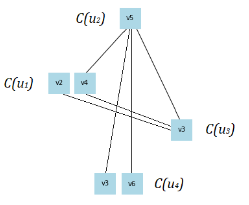
\includegraphics{figures/initcs.png}
        \caption{Initial CS structure}
        \label{fig:dafinitcs}
    \end{figure}

    We use $q' = q^{-1}_D$ for our first refinement. The first vertex will be $u_2$ because it has no children, thus $C'(u_2) = \{v_5\}$
    The second vertex to be processed is $u_1$ because all its children ($u_2$) has been processed already. $v_2$ is not connected with
    any of the candidates of $u_2$. Because of this, $v_2$ will no longer be part of $u_1$'s candidates: $C'(u_1) = \{v_4\}$. The next
    vertex is $u_4$, because its children $u_2$ has been processed. Its new candidates are $C'(u_4) = \{v_3, v_6\}$. The last vertex is
    $u_3$, for which $C'(u_3) = \{v_3\}$. Figure \ref{fig:dafrefcs} shows the CS structure after the first refinement.

    \begin{figure}[h!]
        \centering
        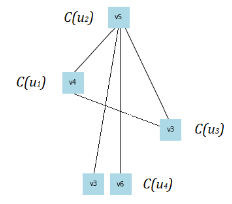
\includegraphics{figures/refinedcs.png}
        \caption{CS structure after the first refinement}
        \label{fig:dafrefcs}
    \end{figure}

    Now $q' = q_D$, however it is not possible to refine CS any further. Next, we find all mappings in CS. The first elements of the 
    search tree is $u_2$ and its candidate ($u_2, v_5$). The set of extendable vertices is $\{u_1, u_4\}$ because their only parent
    $u_2$ in $q_D$ has been processed. We compute the appropriate candidates:

    \[ C_m(u_1) = \{v_4\} \]
    \[ C_m(u_4) = \{v_3, v_6\} \]

    Because of the candidate-size order, we extend the search tree with $u_1$ and its candidate $(u_1, v_4)$. At this point, $u_3$ 
    becomes extendable because its parents were procesed. Its candidates are $C_m(u_3) = \{v_3\}$, and since it is the only extendable
    vertex at the moment, we extend the search tree with $(u_3, v_3)$. The only vertex left is $u_4$. $C_m(u_4) = \{v_3, v_6\}$. The
    search tree is extended with $(u_4, v_3)!$ ($v_3$ is already covered, hence the exclamation mark) and $(u_4, v_6)$. The branch
    containing $(u_4, v_6)$ corresponds to a whole mapping. The failing sets of all nodes on this branch will be empty. The failing set
    of $(u_4, v_3)!$ is $F_m = \{u_3, u_4\}$. In this case, failing sets have no effect on the algorithm. Figure \ref{fig:dafst} shows 
    the search tree with failing sets produced by DAF.

    \begin{figure}[h!]
        \centering
        
        \begin {tikzpicture}[auto, node distance=1cm,thick,main node/.style={circle,draw}]
        \node[main node,label={\scriptsize $F_m = \emptyset$}] (A) {\scriptsize$u_2,v_5$};
        \node[main node,label={\scriptsize $F_m = \emptyset$}] (B) [below=of A] {\scriptsize$u_1,v_4$};
        \node[main node,label={\scriptsize $F_m = \emptyset$}] (C) [below=of B] {\scriptsize$u_3,v_3$};
        \node[main node,label={\scriptsize $F_m = \emptyset$}] (D) [below right =of C] {\scriptsize$u_4,v_6$};    
        \node[main node,red,label={\scriptsize $F_m = \{u_3, u_4\}$}] (E) [below left =of C] {\scriptsize$u_4,v_3!$};    
        \draw (A) -- (B);
        \draw (B) -- (C);
        \draw (C) -- (D);
        \draw (C) -- (E);
        \end{tikzpicture}
        
        \caption{Search tree with failing sets created by DAF}
        \label{fig:dafst}
    \end{figure}

    We got as a result that $q$ is isomorphic to one of $G$'s subgraph and the mapping is the following: $(u_1, v_4),(u_2, v_5),(u_3, v_3),(u_4, v_6)$.

\end{example}

\chapter{Incremental algorithms}

This chapter describes two incremental algorithms for finding subgraph isomorphisms
in dynamic graphs. First we introduce the approach proposed in []. Then we present
our generic method which can be applied to DAF and VF2++ respectively.



\section{Locality based method}

Let \(d\) denote the diameter of the query graph \(q\) which corresponds to the 
length of the longest shortest path in $q$. Let $\Delta e$ denote the addition or
deletion of edge $e = (v, v')$ in $G$. Moreover let $V(d, e)$ be the set of vertices
in $G$ that are within a distance $d$ from $v$ or $v'$. Finally, let $G(d, e)$
be the subgraph of $G$ induced by $V(d, e)$, and $\Delta G(d, e)$ be the subgraph
of $\Delta G$ induced by $V(d, e)$, where $\Delta G = (V, E \setminus \{e\})$ or
$\Delta G = (V, E \cup \{e\})$ depending on the operation of $\Delta e$. With these
notations, we can define the locality property of subgraph isomorphism. For any 
given changes of $\Delta e$ in $G$, the changes $\Delta M$ in the set of mappings
$M(q, G)$ is the difference between $M(q, G(d, e))$ and $M(q, \Delta G(d, e))$, i.e.
the difference between the mappings found in the $d$th neighborhood of the original graph
and in the neighborhood's modified version. This is a trivial property because new mappings can 
appear or become obsolete only in the immediate vicinity of the affected edge $e$. 
Mappings further away from $e$ than $d$ are not affected by $\Delta e$ because neither 
vertices of $e$ are reachable from there. Regardless of that a new edge was added
or an old one was removed, mappings can both appear and become obsolete in the updated
graph. The mappings that have to be added to the existing set is 
$M(q, \Delta G(d, e)) \setminus M(q, G(d, e))$, while the mappings that have to be
removed are $M(q, G(d, e)) \setminus M(q, \Delta G(d, e))$.

The algorithm uses this locality property as follows. Given a query graph $q$ and a 
data graph $G$, compute the initial set of mappings $M$ with a classic subgraph 
isomorphism algorithm, e.g. VF2++. Then, for each update $\Delta e$, (1) find the 
diameter $d$ of $q$, (2) extract the subgraph $\Delta G(d, e)$ from $G$, (3) compute 
$M(q, \Delta G(e, d))$, (4) then update $M$ as described above.

\SetKwComment{Comment}{/* }{ */}

\begin{algorithm}
\caption{Locality algorithm}\label{alg:two}
\KwIn{$q, G, \Delta e, M = VF2++(q, G)$}
$d \gets diameter(q)$\;
$G_{d, e} \gets G(d, e)$\;
$\Delta M \gets VF2++(q, G_{d, e})$\;
$M = M \cup M(q, \Delta G(d, e)) \setminus M(q, G(d, e))$\;
$M = M \setminus M(q, G(d, e)) \setminus M(q, \Delta G(d, e))$\;
\KwRet{$M$}
\end{algorithm}

Instead of re-computing all mappings in $G$, this method works on a subset of $G$.
Although a regular subgraph isomorphism is running in the background, reducing the
size of the input data graph can make this variant faster. The effectiveness depends
on the query graph and the data graph. If $G(d, e)$ remains small compared to $G$,
there will be a massive speed up. However if $G(d, e) \sim G$, for example in case of
small world networks, the algorithm performs the same as a regular subgraph isomorphism
algorithm.


\section{Search tree based method}

This chapter describes our method of making the previously introduced algorithms
incremental. One way or another, both algorithms traverse a search tree eventually.
In both cases the search tree is purely abstract, it has no physical manifestation
in the memory whatsoever. We propose to store the traversed search tree while running
subgraph isomorphism initially, and make use of it in future updates. $T_{q, G}$ is a
search tree of query graph $q$ and data graph $G$, where paths from the root to a leaf
correspond to (partial) mappings, and a node contains an $(u, v)$ pair where 
$u \in V_q, v \in V_G$ denotes a single vertex mapping. The root $r$ of $T_{q, G}$
contains an empty mapping. A root-to-leaf path, whose length $l = |V_q|$ is a complete
mapping because it maps all nodes of $q$. The rest of the root-to-leaf paths correspond
to partial mappings.

In a typical scenario at the end of an execution of a subgraph isomorphism algorithm,
the search tree contains some complete mappings and orders of magnitude more partial 
mappings that for some reason could not be extended any further. These partial mappings 
play a crucial role in the incremental version. One can think about them as potential 
partially precalculated mappings. The reason, why a partial mapping could not be extended
is because the algorithm ran out of valid candidates in the area of the mapped nodes' 
neighborhood in \(G\). This is caused because by some kind of conflict between the 
topology of \(q\) and the topology of the mapped nodes and their neighborhood. These 
conflicts could be resolved when a new edge is added to or an old one is deleted from 
\(G\). At this point, having these partial mappings in memory can speed up the process 
of removing  matches that became obsolete and finding new ones that were impossible in 
the past.

In the upcoming sections, we define an incremental algorithm for each type of graph 
modifications.

\subsection{Node deletion}

Deleting a node from $v_d$ from $G$ can only reduce the original number of mappings.
Mappings that did not contain $v_d$ are unaffected, while those that contained $v_d$ 
have to be removed since they no longer can map to $v_d$. Now we only have to think 
through that no new mappings could arise. Indeed, that cannot be the case because
the only edges that were removed are edges belonging to $v_d$ which means only 
partial mappings which contain $v_d$ are affected. However since $v_d$ itself is also
deleted, these mappings become obsolete, which means that no new mappings can be
found.

Since there are no new mappings to be found, the only work to do in case of a node
deletion is pruning the search tree $T_{q, G}$. More specifically, cut off every
sub-branch that starts with a node $(u, v)$ where $v = v_d$. In worst case scenario
this would mean traversing the whole search space. We already saw however, that any
given change can only affect mappings whose vertices are in the $d$th neighborhood
$N_d(G, v_d)$ of $v_d$. Thus we can skip any branches that map a query graph vertex
to a node $v \notin N_d(G, v_d)$.

\begin{algorithm}[htp]
    \SetAlgoLined\DontPrintSemicolon
    \SetKwFunction{proc}{delete\_node}
    \KwIn{$q, G, T_{q, G}, v_d$}
    \nl $d \gets $ diameter($q$)\;
    \nl $N_d(G, v_d) \gets$ $d$th neighborhood of $v_d$ in $G$\;
    \SetKwProg{myproc}{Procedure}{}{}
    \myproc{\proc{node, $v_d$}}{
        \ForEach(){child $\in$ node.children}{
            \nl $(u, v) \gets $ child.mapping\;
            
            \uIf{$v = v_d$}{
                \nl node.remove(child)\;
            }
            \ElseIf(){$v \in N_d(G, v_d)$}{
                \nl \proc{child, $v_d$}\;
            }
        }
    }
    \caption{Delete node incrementally}
\end{algorithm}

\subsection{Node insertion}

Inserting a new node has no effects on mappings whatsoever because at the time of insertion,
it cannot be part of any mappings because it has not connections. Thus inserting a new node
needs no special care.

\subsection{Edge operations}

In case of induced subgraph isomorphism, both inserting and deleting an edge can result 
in loosing and gaining mappings. Removing an edge $e$ makes mappings where nodes of $e$
were part of the mapping no longer valid. At the same time, in case of partial mappings
where $e$ made it impossible to further extend, removing it may cause new mappings to
appear. For example in \ref{fig:insdelmap}, as a result of removing the BD edge from $G$,
$M(q_1, G')$ will loose half of its mappings, while $M(q_2, G')$ will double the amount of
its mappings. 

\begin{figure}[h]
    \centering
    \begin{subfigure}{.2\textwidth}
      \centering
      \begin {tikzpicture}[auto, node distance=1cm,thick,main node/.style={circle,draw}]
        \node[main node] (A) {\scriptsize$A$};
        \node[main node] (B) [below=of A] {\scriptsize$B$};
        \node[main node] (C) [right =of B] {\scriptsize$C$};
        \node[main node] (D) [right =of A] {\scriptsize$D$};    
        \draw (A) -- (B);
        \draw (B) -- (C);
        \draw (C) -- (D);
        \draw (D) -- (A);
        \draw (A) -- (C);
        \draw[red] (B) -- (D);    
      \end{tikzpicture}
      \caption{$G$}
      \label{fig:sfig1}
    \end{subfigure}%
    \begin{subfigure}{.2\textwidth}
      \centering
      \begin {tikzpicture}[auto, node distance=1cm,thick,main node/.style={circle,draw}]
        \node[main node] (A) {\scriptsize$1$};
        \node[main node] (B) [below=of A] {\scriptsize$2$};
        \node[main node] (C) [right =of B] {\scriptsize$3$};
        \node[main node] (D) [right =of A] {\scriptsize$4$};    
        \draw (A) -- (B);
        \draw (B) -- (C);
        \draw (C) -- (D);
        \draw (D) -- (A);
        \draw (B) -- (D);    
      \end{tikzpicture}
      \caption{$q_1$}
      \label{fig:sfig2}
    \end{subfigure}
    \begin{subfigure}{.2\textwidth}
        \centering
        \begin {tikzpicture}[auto, node distance=1cm,main node/.style={circle,draw}]
          \node[main node] (A) {\scriptsize $1$};
          \node[main node] (B) [below=of A] {\scriptsize $2$};
          \node[main node] (C) [right =of B] {\scriptsize $3$};
          \node[main node] (D) [right =of A] {\scriptsize $4$};    
          \draw (A) -- (B);
          \draw (B) -- (C);
          \draw (C) -- (D);
          \draw (D) -- (A);
        \end{tikzpicture}
        \caption{$q_2$}
        \label{fig:sfig3}
    \end{subfigure}
    \begin{subfigure}{.2\textwidth}
        \centering
        \begin {tikzpicture}[auto, node distance=1cm,main node/.style={circle,draw}]
          \node[main node] (A) {\scriptsize $1$};
          \node[main node] (B) [below=of A] {\scriptsize $2$};
          \node[main node] (C) [right =of B] {\scriptsize $3$};
          \draw (A) -- (B);
          \draw (B) -- (C);
          \draw (C) -- (A);
        \end{tikzpicture}
        \caption{$q_2$}
        \label{fig:sfig4}
    \end{subfigure}
    \caption{Example how mappings can appear and disappear in both cases of edge deletion and insertion.}
    \label{fig:insdelmap}
\end{figure}

The same goes for edge insertion. If we were to insert the BD edge into $G$ then
$M(q_1, G')$ would find new mappings, while $M(q_2, G')$ should remove the half 
of them. It is clear that these can happen simultaneously, as well.

\subsubsection{Edge deletion}

When an edge $e = (v_1, v_2)$ is removed from $G$, first, we have to prune the search
tree to remove mappings that are no longer valid and we have to somehow find the new 
mappings. We have to prune all branches that correspond to a partial mapping which both
$v_1$ and $v_2$ are part of, and there is an edge between $m^{-1}(v_1)$ and $m^{-1}(v_2)$ 
in $q$. We find all paths that correspond to such partial mappings, and prune them down
from the first point where $v_1$ and $v_2$ both appeared in the path. \ref{alg:deledgeprune}
shows the pruning algorithm when an edge was deleted.

\begin{algorithm}[htp]
    \SetAlgoLined\DontPrintSemicolon    
    \SetKwFunction{prune}{prune}
    
    \SetKwProg{pruneproc}{Procedure}{}{}
    \pruneproc{\prune{node, $v_1$, $v_2$}}{
        \nl $(u, v) = $ node.mapping\;
        \uIf(){$v_1$ not marked as found $\wedge$ $v = v_1$}{
            \nl mark $v_1$ as found\;
        }
        \ElseIf(){$v_2$ not marked as found $\wedge$ $v = v_2$}{
            \nl mark $v_2$ as found\;
        }

        \If{$v_1$ is marked $\wedge$ $v_2$ is marked}{
            \If{$(m^{-1}(v_1), m^{-1}(v_2)) \in E_q$}{
                \nl \KwRet{true}\;
            }
        }

        \nl $node.children = \{child \in node.children: \neg \prune(child, v_1, v_2) \}$\;     
    }    
    \caption{Prune search tree on edge deletion}
    \label{alg:deledgeprune}
\end{algorithm}

Fig \ref{fig:pruneex} shows an example partial search tree of $G$ and $q_3$ from Fig. \ref{fig:insdelmap}.
The red nodes represent the pruned sub-branches as a result of removing the $BD$ edge from $G$.

\begin{figure}[h]
    \centering    
    \begin {tikzpicture}[auto, node distance=1cm,main node/.style={circle,draw}]
        \node[main node] (S) {\scriptsize $\emptyset, \emptyset$};
        \node[main node] (R) [below=of S] {\scriptsize $1, B$};
        \node[main node] (A) [below left=of R,red] {\scriptsize $2, D$};
        \node[main node] (AA) [below left=of A,red] {\scriptsize $3, A$};    
        \node[main node] (AB) [below right=of A,red] {\scriptsize $3, C$};    
        \node[main node] (B) [below right=of R] {\scriptsize $2, A$};    
        \node[main node] (BB) [below right=of B] {\scriptsize $3, C$};    
        \draw (S) -- (R);
        \draw (R) -- (A);
        \draw (R) -- (B);
        \draw (A) -- (AA);
        \draw (A) -- (AB);        
        \draw (B) -- (BB);
    \end{tikzpicture}
    \caption{Pruning of a partial search tree of $G$ and $q_3$ from Fig. \ref{fig:insdelmap}.}
    \label{fig:pruneex}
\end{figure}

Finding new mappings is somewhat harder because we have to extend the search tree instead
of just pruning it. Because of the locality property of the incremental subgraph isomorphism
problem, we know for sure that any new mappings that will appear have to contain either $v_1$
or $v_2$ or both. Thus our job is reduced to look for partial mappings that contain either of 
those two vertices. There are two kinds of partial mappings to consider. Typically, the search
tree will contain some partial mappings that contain one of these two vertices but definitely
not all of them. As a first step, we add these partial mappings to the search tree. We traverse 
the tree and check if a node has a child that maps the next vertex $u \in q$ to $v_i$. If it does
not, and $v_i$ was not covered already in the mapping, and it causes no conflicts between the 
topology of the mapping and $q$ then we create a new child under the current node with 
$m(u) = v_i$. Now that we have all the partial mappings containing $v_1$ or $v_2$ - note that not 
all of them are expanded yet - we find all those leaves whose path from the root corresponds to a 
partial mapping that contains $v_1$ or $v_2$ and we execute our choice of subgraph isomorphism 
algorithm from that point. Naturally, these two steps can be combined into one traversal. If we 
hit a node where (1) we can create a new child or (2) a node is a leaf and its path contains $v_1$ 
or $v_2$, and it is not a complete mapping, we execute our subgraph isomorphism algorithm. We
can speed up the algorithm by only considering those branches that contain vertices such that
$\forall v \in m: v \in N_d(G, v_1) \cup N_d(G, v_2)$, i.e. branches that contain only mapped 
vertices such that they are in the $d$th neighborhood of $e$. Alg. \ref{alg:deledgefind}
formally describes the algorithm of finding new mappings after an edge has been deleted, and
Alg. \ref{alg:deledge} shows the incremental algorithm for subgraph isomorphism in case of edge 
deletion.

\begin{algorithm}[ht]
    \SetAlgoLined\DontPrintSemicolon    
    \SetKwFunction{find}{find\_mappings}
    
    \SetKwProg{findproc}{Procedure}{}{}
    \findproc{\find{node, forced\_candidates}}{
        \uIf{node.depth $=$ $|V_q|$ $\lor$ node.mapping.v $\notin N_d(G, (v_1, v_2))$}{
            \nl \KwRet{}\;
        }        

        \nl u $\gets$ node.extendable\_vertex\_of\_children\;
        \ForEach(){$v_c \in forced\_candidates$}{
            \uIf{$\nexists child: child.mapping = (u, v_c)$}{
                \uIf(){$v_c$ is not covered $\wedge$ $v_c$ is good candidate}{
                    \nl child = node.add\_child(u, $v_c$)\;
                    \nl ISO(child)\;
                }
            }
        }
        
        \uIf(){node is leaf $\land$ $(v_1 \in m \lor v_2 \in m)$}{
            \nl ISO(node)\;
        }
        \Else{
            \ForEach(){child $\in$ node.children}{
                \nl \find(child, forced\_candidates)\;
            }
        }

    }        
    \caption{Find new mappings incrementally}
    \label{alg:deledgefind}
\end{algorithm}

\begin{algorithm}[ht]
    \SetAlgoLined\DontPrintSemicolon    
    \SetKwFunction{prune}{prune}
    \SetKwFunction{find}{find\_mappings}
    \KwIn{$q, G, T_{q, G}, e$}
    
    \nl $d \gets $ diameter($q$)\;
    \nl $(v_1, v_2) = e$\;
    \nl $N_d(G, (v_1, v_2)) \gets$ $d$th neighborhood of $v_1$ and $v_2$ in $G$\;
    \nl \prune(root($T_{q, G}$), $v_1, v_2$)\;
    \nl \find(root($T_{q, G}$), $\{v_1, v_2\}$)\;    
    
    \caption{Delete edge incrementally}
    \label{alg:deledge}
\end{algorithm}


\subsubsection{Edge insertion}

Inserting a new edge into $G$ will have a really similar effect on the mappings as and edge
deletion. Mappings can both appear and disappear from the original mapping set. In fact, the
algorithm described above is almost applicable to this problem out of the box. It is clear 
that finding new mappings will be the same in this case, as well. We have to take care about
how we prune the search tree before that. Indeed, removing nodes that pass the test 
$(m^{-1}(v_1), m^{-1}(v_2)) \in E_q$ makes no sense because we just added that new edge. We
can make this condition generic however, so that both edge operations can use the same predicate.
Instead of separating the two cases, we will simply check that an edge between $v_1$ and $v_2$
in $G$ exists if and only if an edge between $m^{-1}(v_1)$ and $m^{-1}(v_2)$ in $q$ exists.
With these modifications, the final pruning algorithm can be found in Alg. \ref{alg:edgeprune}.

\begin{algorithm}[ht]
    \SetAlgoLined\DontPrintSemicolon    
    \SetKwFunction{prune}{prune}
    
    \SetKwProg{pruneproc}{Procedure}{}{}
    \pruneproc{\prune{node, $v_1$, $v_2$}}{
        \nl $(u, v) = $ node.mapping\;
        \uIf(){$v_1$ not marked as found $\wedge$ $v = v_1$}{
            \nl mark $v_1$ as found\;
        }
        \ElseIf(){$v_2$ not marked as found $\wedge$ $v = v_2$}{
            \nl mark $v_2$ as found\;
        }

        \If{$v_1$ is marked $\wedge$ $v_2$ is marked}{
            \nl is\_edge\_in\_q $\gets$ $(m^{-1}(v_1), m^{-1}(v_2)) \in E_q$\;
            \nl is\_edge\_in\_G $\gets$ $(v_1, v_2) \in E_G$\;
            \If{is\_edge\_in\_q $\neq$ is\_edge\_in\_G}{
                \nl \KwRet{true}\;
            }
        }

        \nl $node.children = \{child \in node.children: \neg \prune(child, v_1, v_2) \}$\;     
    }    
    \caption{Prune search tree on edge operation}
    \label{alg:edgeprune}
\end{algorithm}
\chapter{Evaluation}

In this chapter, we evaluate our version of incremental induced subgraph isomorphism algorithms.

\subsection{Implementation details}

All algorithms were written in Python. Although Python is not necessarily the right tool 
for implementing high performance algorithms, the main goal of this work was to verify if
we can make significant improvements compared to running VF2++/DAF from scratch by computing
mappings incrementally. To evaluate the correctness of our work, two already existing induced 
subgraph isomorphism implementations were used: networkx's (Python graph library) isomorphism 
module and boost c++ library's vf2\_subgraph\_iso module\cite{boostvf2}. Both modules implement VF2. We 
tried to compare the performance against the original VF2++ implementation \cite{lemonvf2pp}
however it did not produce the same results as the selected baseline implementations. We also
wanted to compare our results to the original DAF implementation, however no sources for the
project were available at time of writing, only a set of pre-compiled binaries \cite{dafbin}
which we did not want to run in the end.

\subsection{Datasets}

We used multiple datasets in our experiments. The first dataset was the Graph Challange\cite{graphchallenge} dataset
which was published by Massachusetts Institute of Technology (MIT) and Amazon Web Services for
the challange. The dataset consists of several large graphs. 

\begin{itemize}
    \item as: network of autonomous systems.
    \item ca-GrQc: collaboration network of general relativity researchers on arxiv.org.
    \item ca-HepTh: collaboration network of high energz physics researchers on arxiv.org.
    \item iso-m2D-m196.A00
    \item iso-m2D-m196.A01
    \item oregon1: peering infromation of autonomous systems in project Route Views of University of Oregon.
\end{itemize}

The other dataset contains multiple generated graphs, namely

\begin{itemize}
    \item random graphs with 1000 nodes and different number of edges between 1500 and 50000. 
    \item scale-free networks generated by the Barabasi-Albert model\cite{barabasimodel}.
\end{itemize}

\subsection{Measurements}

For each of the graphs, the following operations were made. We ran an initial VF2++ and DAF on the given graph $G$
with query graph defined in figure \ref{fig:expq}. Then we randomly deleted and inserted nodes and edges into $G$,
and we measured how much time does it take to incrementally compute the new mapping set. After the graph modifications
we ran our baseline measurement on the resulting graph $G'$, which was networkx's VF2 implementation and we measured
the time it took for the algorithm to finish. We also verified that the number of ismorphisms found by all algorithms
were the same.

\begin{figure}[h!]
	\centering
	\begin {tikzpicture}[auto, node distance=1cm,thick,main node/.style={circle,draw}]
		\node[main node] (0) {\scriptsize$0$};
		\node[main node] (1) [below left=of 0] {\scriptsize$1$};
		\node[main node] (2) [below right=of 0] {\scriptsize$2$};
		\node[main node] (3) [below=of 1] {\scriptsize$3$};
		\node[main node] (4) [below=of 2] {\scriptsize$4$};
		\draw (0) -- (1);
		\draw (0) -- (2);
		\draw (1) -- (2);
		\draw (2) -- (4);
		\draw (3) -- (4);
		\draw (1) -- (3);
	  \end{tikzpicture}
	\caption{Query graph for our experiments}
	\label{fig:expq}
\end{figure}

The first step of our incremental algorithm is to run VF2++ and DAF from scratch. As expected, both algorithms are generally 
faster than VF2. More importantly, the results verify our proposed algorithm. It is significantly faster to update a graph and
incrementally search changes in the mappings set than running a subgraph ismorphism algorithm from scratch. This applies to all
kinds of graphs, even where all three variants semm to struggle, the incremental version still finishes at least one order of
magnitudes earlier.

\begin{figure}
	\begin{tikzpicture}
		% let both axes use the same layers
		\pgfplotsset{set layers}
		%
		\begin{axis}[
		scale only axis,
		xmin=0,xmax=1,
		xtick={0,1},
        xticklabels={ca-GrQc,ca-HepTh},
		axis y line*=left,
		ylabel style = {align=center},
		ylabel={Initial VF2++ \ref{plot:vf2ppinitca} \\ networkx VF2 \ref{plot:nxca}},
		]
		\addplot[
            color=blue,
            mark=square,
            ]
            coordinates {
            (0,35.7)(1,54.1)
            };
			\label{plot:vf2ppinitca}
		\addplot[
			color=red,
			mark=square,
			]
			coordinates {
			(0,20)(1,80)
			};
			\label{plot:nxca}
		
		\end{axis}
		%
		\begin{axis}[
		scale only axis,
		xmin=0,xmax=1,
		axis y line*=right,
		axis x line=none,
		ylabel style = {align=center},
		ylabel={Avg. VF2++ delete node \ref{plot:avgnodeca} \\ Avg. VF2++ insert/delete edge \ref{plot:avginsca}},
		]
		\addplot[
			color=green,
            mark=square,
            ]
            coordinates {
            (0,0.62)(1,0.57)
            };
            \label{plot:avgnodeca}
        \addplot[
			color=orange,
            mark=square,
            ]
            coordinates {
            (0,7.48)(1,6.46)
            };
            \label{plot:avginsca}
		\end{axis}
		%
		\end{tikzpicture}
		\caption{Results of ca graphs from Graph Challange}
\end{figure}

\begin{figure}
	\begin{tikzpicture}
		% let both axes use the same layers
		\pgfplotsset{set layers}
		%
		\begin{axis}[
		scale only axis,
		xmin=0,xmax=2,
		xtick={0,1,2},
        xticklabels={oregon1\_010331,oregon1\_010407, oregon1\_010414},
		axis y line*=left,
		ylabel style = {align=center},
		ylabel={Initial VF2++ \ref{plot:vf2ppinitoregon} \\ networkx VF2 \ref{plot:nxoregon}},
		]
		\addplot[
            color=blue,
            mark=square,
            ]
            coordinates {
            (0,1595)(1,2763)(2,3401)
            };
			\label{plot:vf2ppinitoregon}
		\addplot[
			color=red,
			mark=square,
			]
			coordinates {
			(0,4896)(1,5217)(2,5579)
			};
			\label{plot:nxoregon}		
		\end{axis}
		%
		\begin{axis}[
		scale only axis,
		xmin=0,xmax=1,
		axis y line*=right,
		axis x line=none,
		ylabel style = {align=center},
		ylabel={Avg. VF2++ delete node \ref{plot:avgnodeoregon} \\ Avg. VF2++ insert/delete edge \ref{plot:avginsoregon}},
		]
		\addplot[
			color=green,
            mark=square,
            ]
            coordinates {
            (0,35.94)(1,46.87)(2,58.77)
            };
            \label{plot:avgnodeoregon}
        \addplot[
			color=orange,
            mark=square,
            ]
            coordinates {
            (0,179.54)(1,198.03)(2,236.77)
            };
            \label{plot:avginsoregon}
		\end{axis}
		%
		\end{tikzpicture}
		\caption{Results of oregon graphs from Graph Challange}
\end{figure}

\begin{figure}
	\begin{tikzpicture}
		% let both axes use the same layers
		\pgfplotsset{set layers}
		%
		\begin{axis}[
		scale only axis,
		xmin=500,xmax=4500,
		xtick={500,1000,...,4500},
		axis y line*=left,
		ylabel style = {align=center},
		ylabel={Initial VF2++ \ref{plot:vf2ppinitbar} \\ networkx VF2 \ref{plot:nxbar}},
		]
		\addplot[
            color=blue,
            mark=square,
            ]
            coordinates {
            (500,0.34)(1000,0.77)(1500,1.02)(2000,2.19)(2500,3.03)(3000,3.13)(3500,4.096)(4000,3.46)(4500,4.38)
            };
			\label{plot:vf2ppinitbar}
		\addplot[
			color=red,
			mark=square,
			]
			coordinates {
			(500,3.97)(1000,9.2)(1500,12.85)(2000,21.48)(2500,38.05)(3000,37.74)(3500,41.91)(4000,36.26)(4500,53.33)
			};
			\label{plot:nxbar}		
		\end{axis}
		%
		\begin{axis}[
		scale only axis,
		xmin=500,xmax=4500,
		axis y line*=right,
		axis x line=none,
		ylabel style = {align=center},
		ylabel={Avg. VF2++ delete node \ref{plot:avgnodebar} \\ Avg. VF2++ insert/delete edge \ref{plot:avginsbar}},
		]
		\addplot[
			color=green,
            mark=square,
            ]
            coordinates {
            (500,0.0101)(1000,0.0245)(1500,0.02669)(2000,0.0433)(2500,0.0711)(3000,0.0661)(3500,0.0739)(4000,0.0634)(4500,0.0984)
            };
            \label{plot:avgnodebar}
		\addplot[
			color=orange,
			mark=square,
			]
			coordinates {
			(500,0.1425)(1000,0.1994)(1500,0.2462)(2000,0.3623)(2500,0.6001)(3000,0.5653)(3500,0.6199)(4000,0.5104)(4500,0.7201)
			};
			\label{plot:avginsbar}    
		\end{axis}
		%
		\end{tikzpicture}
		\caption{Results of scale-free graphs generated by Barabasi-model}
\end{figure}
\chapter{Future work}

We implemented our algorithms in Python to verify that our approach could work in reality. As stated earlier,
Python in itself is not suited for high performance algorithms. Future works can include implementing these
incremental algorithms in a language which allow more fine-tuned memory handling, e.g. C++.

Since both VF2++ and DAF work on tree structures, both algorithms can be naturally implemented paralelly. This
also applies for our modified incremental algorithm. Future research can involve parallelizing these algorithms.

Another area of future work would be using neural networks for detecting isomorphisms in large graphs. The use 
cases may not fully align with out current work, because statistical approaches can not guarantee to find all
subgraph ismorphisms. However the performance gain might out-weight the issue of missing mappings.
\chapter{Conclusion}

In this work, we introduced a novel incremental algorithm for finding induced subgraph isomorphisms in large dynamic graphs.
The algorithm can be used in cases when there are frequent changes to the data graph. In these use-cases the proposed procedure
out-performs any induced subgraph isomorphism solution run from scratch.

% Acknowledgements
%~~~~~~~~~~~~~~~~~~~~~~~~~~~~~~~~~~~~~~~~~~~~~~~~~~~~~~~~~~~~~~~~~~~~~~~~~~~~~~~~~~~~~~
% %----------------------------------------------------------------------------
\chapter*{\koszonetnyilvanitas}\addcontentsline{toc}{chapter}{\koszonetnyilvanitas}
%----------------------------------------------------------------------------

Ez nem kötelező, akár törölhető is. Ha a szerző szükségét érzi, itt lehet köszönetet nyilvánítani azoknak, akik hozzájárultak munkájukkal ahhoz, hogy a hallgató a szakdolgozatban vagy diplomamunkában leírt feladatokat sikeresen elvégezze. A konzulensnek való köszönetnyilvánítás sem kötelező, a konzulensnek hivatalosan is dolga, hogy a hallgatót konzultálja.


% List of Figures, Tables
%~~~~~~~~~~~~~~~~~~~~~~~~~~~~~~~~~~~~~~~~~~~~~~~~~~~~~~~~~~~~~~~~~~~~~~~~~~~~~~~~~~~~~~
%\listoffigures\addcontentsline{toc}{chapter}{\listfigurename}
%\listoftables\addcontentsline{toc}{chapter}{\listtablename}


% Bibliography
%~~~~~~~~~~~~~~~~~~~~~~~~~~~~~~~~~~~~~~~~~~~~~~~~~~~~~~~~~~~~~~~~~~~~~~~~~~~~~~~~~~~~~~
\addcontentsline{toc}{chapter}{\bibname}
\bibliography{bib/mybib}


% Appendix
%~~~~~~~~~~~~~~~~~~~~~~~~~~~~~~~~~~~~~~~~~~~~~~~~~~~~~~~~~~~~~~~~~~~~~~~~~~~~~~~~~~~~~~
% %----------------------------------------------------------------------------
\appendix
%----------------------------------------------------------------------------
\chapter*{\fuggelek}\addcontentsline{toc}{chapter}{\fuggelek}
\setcounter{chapter}{\appendixnumber}
%\setcounter{equation}{0} % a fofejezet-szamlalo az angol ABC 6. betuje (F) lesz
\numberwithin{equation}{section}
\numberwithin{figure}{section}
\numberwithin{lstlisting}{section}
%\numberwithin{tabular}{section}

%----------------------------------------------------------------------------
\section{A TeXstudio felülete}
%----------------------------------------------------------------------------
\begin{figure}[!ht]
\centering
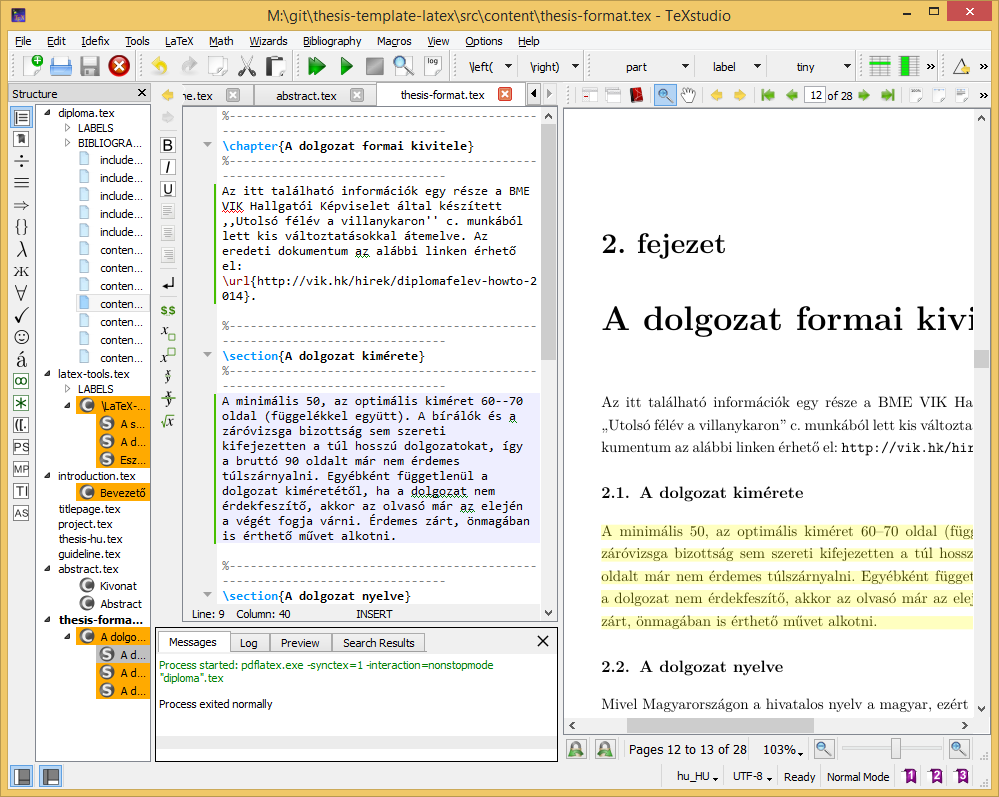
\includegraphics[width=150mm, keepaspectratio]{figures/TeXstudio.png}
\caption{A TeXstudio \LaTeX-szerkesztő.} 
\end{figure}

%----------------------------------------------------------------------------
\clearpage\section{Válasz az ,,Élet, a világmindenség, meg minden'' kérdésére}
%----------------------------------------------------------------------------
A Pitagorasz-tételből levezetve
\begin{align}
c^2=a^2+b^2=42.
\end{align}
A Faraday-indukciós törvényből levezetve
\begin{align}
\rot E=-\frac{dB}{dt}\hspace{1cm}\longrightarrow \hspace{1cm}
U_i=\oint\limits_\mathbf{L}{\mathbf{E}\mathbf{dl}}=-\frac{d}{dt}\int\limits_A{\mathbf{B}\mathbf{da}}=42.
\end{align}


%\label{page:last}
\end{document}
